

\newcommand\rper{$R_{\rm{per}}$}


\chapter{The Intermediate Period Gap}

\section*{Abstract}


Photometric variability due to stellar spots allows astronomers to measure the surface rotation periods of stars.
Within multiple missions' rotational period samples (e.g. \kepler, \ktoo, \ZTF) there is a distinct dearth of observations of stars rotating at intermediate periods 15 $\gtrsim P_{rot} \gtrsim$ 20 days.
This dearth of observations is known as the intermediate period gap.
The position of this gap varies with the colour of the stars.
Various mechanisms have been proposed to explain the dearth of observations from stars physically "jumping" the gap through enhanced wind-braking, to stars above and below the gap representing two populations of stars, to the gap representing a minima of probability to observe rotation rate.
The exact cause of the dearth of observations is currently unknown.
In this Chapter, we show that the gap aligns itself with minima in both the photometric variability range and magnetic activity indicator $\log R^{+}_{\rm{HK}}$.
This suggests that the minima of photometric variability and $\log R^{+}_{\rm{HK}}$ result from the same mechanism.
We also suggest that there is no subsample of stars with uncharacteristically low magnetic activity in the sample of stars without detection rotation periods.
Further, we argue that the number of stars with undetected rotation periods is unlikely to fill the dearth of observations.
We propose that the data suggests that the gap does not represent a minima of observation of stellar rotation through photometric variability.

\newpage

\section{Intoduction}
\label{sec:intro}
Measurement of the rotational period of samples of stars allows us to understand internal mechanisms that we otherwise would not be able to probe.
For example, the mass-dependent core-envelope coupling and decoupling of young stars have only recently been observed by measuring the rotational period of stars with age through the rotational period distribution of clusters \citep{reinhold_rotation_2015-1}.
An unexplained feature of the rotational period distribution of low-mass main-sequence stars comes in the form of what is known as the intermediate period gap.
The intermediate period gap represents a minimum of observations of stars with particular rotation periods dependent on temperature, first observed by \citet{mcquillan_rotation_2014}.
The feature is selection function independent - the gap is robust between different photometric observation missions \citep{mcquillan_rotation_2014,davenport_rotating_2017,davenport_rotating_2018,lu_bridging_2022}, multiple period detection methods and varies its position in period with respect to mass. 
This suggests that the lack of observation of stars is not a quirk in the data or the data analysis process but a physical feature of the stars we are observing.
The quality cuts made to the samples of stars where rotation is attempted to be measured do not appear to be biased away from detecting gap stars.
If the gap aligned itself with a line of constant rotation in only one mission, then the mechanism underlying the gap could be more readily explained through the selection function of said mission.
These factors suggest that the intermediate period gap represents a function of stellar evolution or an unaccounted-for problem in observing rotation periods through photometric oscillations from stellar spots.
The intermediate period gap interests astronomers and astrophysicists because the mechanism underlying it is unexplained.
Therefore, the effects of this process are unknown in stellar evolution.

Multiple mechanisms have been proposed to explain the intermediate period gap.
\citet{mcquillan_rotation_2014} first proposed that the gap represents bimodal bursty star formation in the local \kepler field.
They suggest that the lower rotation period (faster rotators) prong represents a younger population and the upper rotation period prong represents an older population, with the gap representing a minima in star formation at a particular time.
\citet{davenport_rotating_2018} support local bursty star formation hypothesis by separating the \kepler{} rotation period distribution by distance through \gaia{} \ parallaxes.
They find that the gap appears to disappear for stars further away than 525 pc.
They fail to acknowledge, however, that at those distances (a) observations of stars is magnitude-limited to brighter high-mass stars (M $>$0.9 M$_{\odot}$) where observations of the gap are tentative and (b) period detection and temperature/colour measurement are much less precise.
If the gap extends up to these high-mass stars, then its existence can be blurred out by the imprecision of these measurements.
Their work may also support this explanation.
In the full \citep{mcquillan_rotation_2014} sample the gap disappears for high mass ($M_{\odot} > 0.8$, $B_P - R_P < 1.0$) stars.
In the distance limited ($<$ 525pc) sample, the gap appears to permeate to these higher-mass stars. 
This can be seen in the rotational period-colour distribution in the top two panels in Figure 2 of \citet{davenport_rotating_2018} where distance is limited to 525pc.

More recent works significantly disfavour the bursty star formation hypothesis.
\citet{gordon_stellar_2021} detected the gap in multiple pointings of the \ktoo \ mission, while \citet{curtis_when_2020} found that the open cluster Ruprecht 147 contains stars above and below the gap - and the possible detection of a star within the intermediate period gap.
This suggests that the gap is not a coeval feature and rather a feature of the rotational evolution of low-mass stars.
\citet{curtis_when_2020} instead proposed that the gap aligns with a line of constant Rossby number ($R_o\sim 0.6$) - rotation rate scaled quantity shown to be associated with the magnetic activity of stars.

\citep{mcquillan_rotation_2014} suggested another explanation for the intermediate period gap through a rapid spin-down - "jumping" across the gap quickly, resulting in decreased stars' density in this period-colour space region.
For example, the rapid spin-down could be caused by core and convective envelope rotational decoupling at the upper edge of the lower prong near the rotational period gap.
In this mechanism, the core and envelope evolve independently; the envelope - having a much smaller moment of inertia than the core - is spun down rapidly under the same magnetic braking conditions.
Following the gap the core and envelope then recouple, exchanging angular momentum and returning to a normal rate of magnetic braking. 
\citet{gordon_stellar_2021} argued in favour of this hypothesis based on the rotation period distribution of \ktoo{}. 
\citet{curtis_when_2020} argued that two-zone angular momentum transport models, such as those by \citet{spada_competing_2020} can reproduce a stalled braking behaviour required to explain the lower prong of the intermediate rotational period gap - but their model could not explain the rapid-spin down.
This hypothesis is generally supported by the tentative observation of low-mass fully convective stars permeating the gap \citep{lu_bridging_2022}.

\citet{santos_surface_2021} measured the rotation period of stars with lower variability and expanded the upper range of rotation periods that can be observed through \kepler{} data.
They did not find more stars in or around the intermediate period gap than \citet{mcquillan_rotation_2014}, suggesting that the gap is, in fact, empty.
\citet{lu_bridging_2022} examined the kinematic stellar ages below and above the gap.
They tentatively found that the relation between kinematic age and Rossby number of stars above and below the gap is discontinuous (see Figure 11 in their work).
While this result supports the hypothesis that stars could have gone through a phase of rapid spin-down and jumped over the gap, more precise measurement of kinematic ages for more stars is required to support this claim.

On the other hand, \citet{reinhold_transition_2019} and \citet{reinhold_stellar_2020} proposed that a transition from dark spot creates the gap - to bright facula dominance in the activity cycle of a star.
In this work, they differentiate between the rotation brightness modulation and brightness modulation from the stellar activity cycle.
Stellar activity modulation refers to the long-term evolution of average brightness due to stellar spots and faculae rather than variations on the rotational time scale.
They suggest that as a star spins down and the magnetic field topology changes, the initially strong and long-lived spots are replaced by smaller, short-lived spots surrounded by bright faculae.
In such a scenario, the photometric variability amplitude decreases because of the partial cancellation by the increase and decrease in brightness from the faculae and spots, respectively.
Hence, the stars with small photometric variability will not be detected.
This hypothesis is supported by the gap aligning with a line of constant Rossby number - indicative of common magnetic field evolution between these stars - and by the photometric variability reaching a local minimum surrounding the gap.

As of writing there are two separate explanations for the gap.
First, consider that the intermediate rotational period gap represents a sudden onset of extreme rotational braking.
In that case, gap stars represent a laboratory for understanding the evolution of the magnetism in stars, and the underlying mechanism that provides the enhanced wind braking is of interest to the scientific community. 
This enhanced braking would need to be accounted for in gyrochronological models.
On the other hand, let's say that the stars within the gap exist; there are stars with rotational periods that would place them in the gap, but we cannot measure their periods for whatever reason.
If this is the case, we have undoubtedly observed gap stars that we do not know are gap stars.
Therefore, whether gap stars are peculiar - photometrically, spectroscopically or asteroseismically - is unknown.
It is entirely possible, but likely not probable, that gap stars have been previously flagged as peculiar, but the link between the gap and these stars has never been made.
On the other hand, gap stars may not be otherwise peculiar - chemically or, say, in terms of magnetic activity.
If indeed they are not otherwise peculiar, then, oxymoronically, the reason for their lack of observation raises more questions about the mechanism underlying the gap.

In this work, we will use the terms probability of observation of rotation and detectability of rotation period.
While they are related, they are distinct terms.
The detectability of rotation requires a relatively short cadence, on the time scale of days-weeks, observations with distinct variability in the light curve due to spots, or faculae.
It is dependent on a number of factors on a star-to-star basis, including the inclination angle, wherein the magnetic activity cycle observations are made, where faculae and spots are distributed on the surface of the star and the lifetimes of these surface features relative to the rotation period of the star. \citep{aigrain_hare_2015, reinhold_spot_2018, reinhold_where_2021}.
On the other hand, the probability of observation of rotation refers to a more stellar parameter-based average statistic under the comparison of the set of stars with and without detection rotation periods.
The detectability of rotation with fundamental stellar properties (temperature, metallicity, stellar age etc.) has been previously investigated.
Cooler stars, especially cooler than 5,200K are detected in period significantly more than hotter stars.
Cooler stars both tend to have higher magnetic activity, and therefore more spots, and also have larger brightness variations as a result of the same level of surface spot activity compared to hotter stars \citep{ mcquillan_rotation_2014, santos_surface_2020, zhang_magnetic_2020}
A relation with metallicity has also been investigatied \citep{amard_evidence_2020,see_photometric_2021,claytor_recovery_2022}.
Higher-metallicity ([Fe/H] $\gtrsim$ -0.1) stars being detected in period more frequently than lower-metallicity stars.
 \citep{avallone_rotation_2022, masuda_detectability_2022} separate the metallicity dependence from age and suggest that this effect arises from the fact that younger, more active stars are enriched by metals from Galactic chemical evolution rather than an effect of the metallicity on the evolution of magnetic activity and probability of rotational observation.
Older stars tend to have a lower probability of observation - their rotation periods are long and thus require a longer baseline of observations and they tend to have weaker magnetic fields and thus express a smaller number of stellar spots.
Many stars cannot have their rotation periods measured, purely from the effect of the inclination angle on the detectability of rotation
If a star is pole-on, even if a star expresses surface features close to the axis of rotation, no variance in the brightness of that star will be detected.
Increasing the sensitivity of telescopes, and methods of determining rotation periods, increase the number of stars that can have their rotation periods detected but this number is bounded by the subsample of stars that cannot have their rotation measured.
While the distribution of the inclination angle of stars is biased toward equator-on observations, a non-zero population of stars will never have their rotation periods detected through photometric variability.

 
This Chapter is structured as follows. In Section \ref{sec:act_ind} we will introduce the so-called magnetic activity indicators. 
In Section \ref{minima_rper} we reconfirm that the gap aligns itself with a minima in photometric variability range, then in Section \ref{minima_rhk} we show that this minima aligns itself with a minima in $\log R^{+}_{\rm{HK}}$.
We then show, in Section \ref{sec:low_activity_gap}, that the sample of stars with undetected rotation does not contain a subsample of stars with magnetic activity low enough to fall below the rotation-detection threshold.
In Section \ref{sec:no_gap_stars} we show that the number of stars required for the dearth of observations to no longer be considered a dearth requires a larger number of stars than the number of stars within the undetected sample.
Finally in Section \ref{sec:sum_dis} we summarise and discuss the implications of our work on proposed mechanisms to explain the intermediate period gap.


\section{Stellar activity indicators}
\label{sec:act_ind}

Stellar magnetism is a complex component of stellar evolution that is hard to predict and model.
Links between magnetism and mass, metallicity, age, convection, and rotation have been identified \citep{cao_starspots_2022}.
These links are, however, based upon observations of stars rather than astrophysical theory.
The observation of rotational modulation in a light curve, and the observation of surface rotation from that modulation, requires cool spots and bright faculae created by concentrated magnetic fields near the surface of a star.
Stars with stronger magnetic fields tend to express larger spot coverage, thus having larger rotational photometric modulation and more readily observable rotation periods.

Stellar activity is the collective term used to describe different effects magnetic fields have on stars
This name arises from the variability phenomena arising from structured magnetic fields emerging from the convective envelope of stars - for example flares and large-scale photometric variability from stellar surface features (stellar spots or faculae).
The strength of the magnetic field can be directly or indirectly measured in a number of ways and the photometric variance of a star varies with the strength of the magnetic field.

Throughout the stellar atmosphere, emission features arise through the interaction of light and elements. 
Different absorption features arise from both different elements and different stellar atmosphere conditions.
One of the most frequently probed indicators of chromospheric activity, and thus magnetic field strength, in low-mass magnetically active stars is the non-thermal flux reversal in the cores of the Ca II $H$ and $K$ lines at 3968\AA and 3933\AA respectively.
These ions originate in the upper photosphere and chromosphere and are sensitive to magnetic activity.


Two measures of the chromospheric Ca II $H$ and $K$ line fluxes are generally adopted.
First through the classical $S$ index.
This is the flux ratio in the core of the Ca II $H$ and $K$ lines to close by continuous windows
\begin{equation}
S = \alpha \frac{}{H+K}{R+V},
\end{equation}
where $H$ and $K$ are the line fluxes measured in 1.09\AA-wide triangular bandpasses while $R$ and $V$ are estimates of the continuum on either side of the lines measured in 20\AA-wide spectral windows centered on 3901\AA and 4001\AA. 
\alpha is a normalisation constant dependent on the telescope used to make the measurements, providing a link between samples.
The quantity $S$ is sensitive to the integrated emission over these windows. and the photospheric radiation transmitted in the $H$ and $K$ passbands. 
$S$ is therefore evolutionary and metallicity dependent which renders direct comparison of $S$ between different spectral type stars unsuitable.
The quantity $R_{\rm{HK}}^{+}$ eliminates this contribution \citep[See]{citeme} and is thus a more reliable measure of the chromospheric Ca II $H$ and $K$ flux - therefore more accurately reflecting the magnetic field strength of stars and makes the comparison of magnetic activity of stars of different spectral types suitable.

Another indirect measure of the magnetic field's strength arises from the stars photometric variability.
Here we differentiate between the large-scale photometric variability of a star during a magnetic activity cycle, where the average stellar flux of a star increases and decreases over the course of years and the variability range of a star due to stellar spots on a rotational time scale.
The solar integrated Ca II index, $S$, correlates linearly with photospheric sunspot number, Lorenzo-Oliveira et al. established a robust relationship between solar chromospheric activity and the international sunspot number for solar-like stars, suggesting that the two are interconnected. 
However, it is uncertain whether this correlation is strong enough to derive long-term chromospheric activity cycles similar to photometric cycles on magnetic activity timescales (years)
The consistently similar periods of the two relations suggest the two are interconnected - with the faculae or star spot dominance of the magnetic photometric cycles being derived from the expected relation between the two.
A star that expresses stellar spots results in larger photometric variability as a star rotates.
Photometric variability can been measured through various means.
The first is the amplitude of periodic variability, \rper{}.
This is defined as the median of the range between the 5$^{th}$ and 95$^{th}$ percentile of normalised flux in bins of the light-curve divided into sections of the length of the measured rotational period \citep{mcquillan_rotation_2014}.
Larger \rper{} stars are expected to have more easily detectable rotation periods because the larger the star's variability as it rotates, the more easily distinguishable this variability is from noise.

Finally, the most recent measure of stellar activity has arisen from the measurement of the fractional spot coverage of stars (See Chapter \ref{chap:stellar_spots} and \citep{cao_starspots_2022}).
They found that fitting APOGEE spectra with two temperature components allows one to infer the surface fractional spot coverage and the temperature contrast of the spots to the ambient surroundings.
The stellar spot expression of stars is expected to be tied to the photometric variability of those stars with larger photometric variability arising from a larger fractional spot coverage.

All of these measurements of magnetic activity have been shown to be related to each other and follow similar relations with the stellar Rossby number.
Magnetic activity tends to saturate below a $R_o<0.3$ \citep{cao_starspots_2022} (fast rotation) and decrease with a power law as $R_o$ increases.
This relation reflects the decreased probability of observing older slow-rotating stars in the \citet{mcquillan_rotation_2014} sample.
Variations to magnetic activity can therefore indicate variations to the expression of stellar spots and, thus, the observability of stellar rotation.

The magnetic activity also varies with the stellar magnetic cycle of a star, with some scatter to magnetic activity indicators being attributed to this.
Therefore, a single temporal measurement of magnetic activity must be treated with care.
Variations to the magnetic activity of stars, in a population-wide sense, should be found by the average magnetic activity of a sub-population.
In this work we adopt this average, population study approach, to minimise this effect.

\section{The gap aligns with a minima in photometric variability}
\label{sec:minima_rper}

The first mechanism we consider is that the rotation period gap reflects a decrease in photometric variability due to a variation in the magnetic field strength of stars near the gap.
We will begin with the 33,000 stars with rotation periods from \citet{mcquillan_rotation_2014}.
While this sample has been superseded by other missions in terms of sensitivity, the increase in sensitvity has \textit{not} increased the number of detected rotation periods with large $B_P - R_P$ (lower mass) where the gap is most apparent.
It is still the state-of-the-art mission for precise measurement of the rotation periods of low-mass stars near the intermediate period gap.
All stars in this sample lay within the cross-match with \gaia data release 3, which contains precise measurements of the $B_P - R_P$ colour, $G$-band magnitude and distance from parallax.
We limit our sample to stars within the nearest 525pc, motivated by the results of \citet{davenport_rotating_2018}.
While this reduces the sample to 8,594 stars it ensures that the measured $B_P - R_P$ and rotation periods are as accurate as possible.
% \todo{Add figure of the cuts}
We made cuts in Gaia DR3 magnitudes and colours using $M_G$ $>$ 0 and $B_P - R_P > 0.8$ to target below the main-sequence turnoff and stars lower mass than the Kraft Break.
This leaves us with a sample of 6,243 nearby stars with reliable surface rotation and colour measurements.
These stars are shown in Figures \ref{fig:hr} and \ref{fig:prawn} where we have plotted them as a HR diagram and log rotation period against $B_P-R_P$ colour.
In Figure \ref{fig:prawn} the decrease in photometric variability surrounding the gap can be clearly seen.

\begin{figure}
\centering
    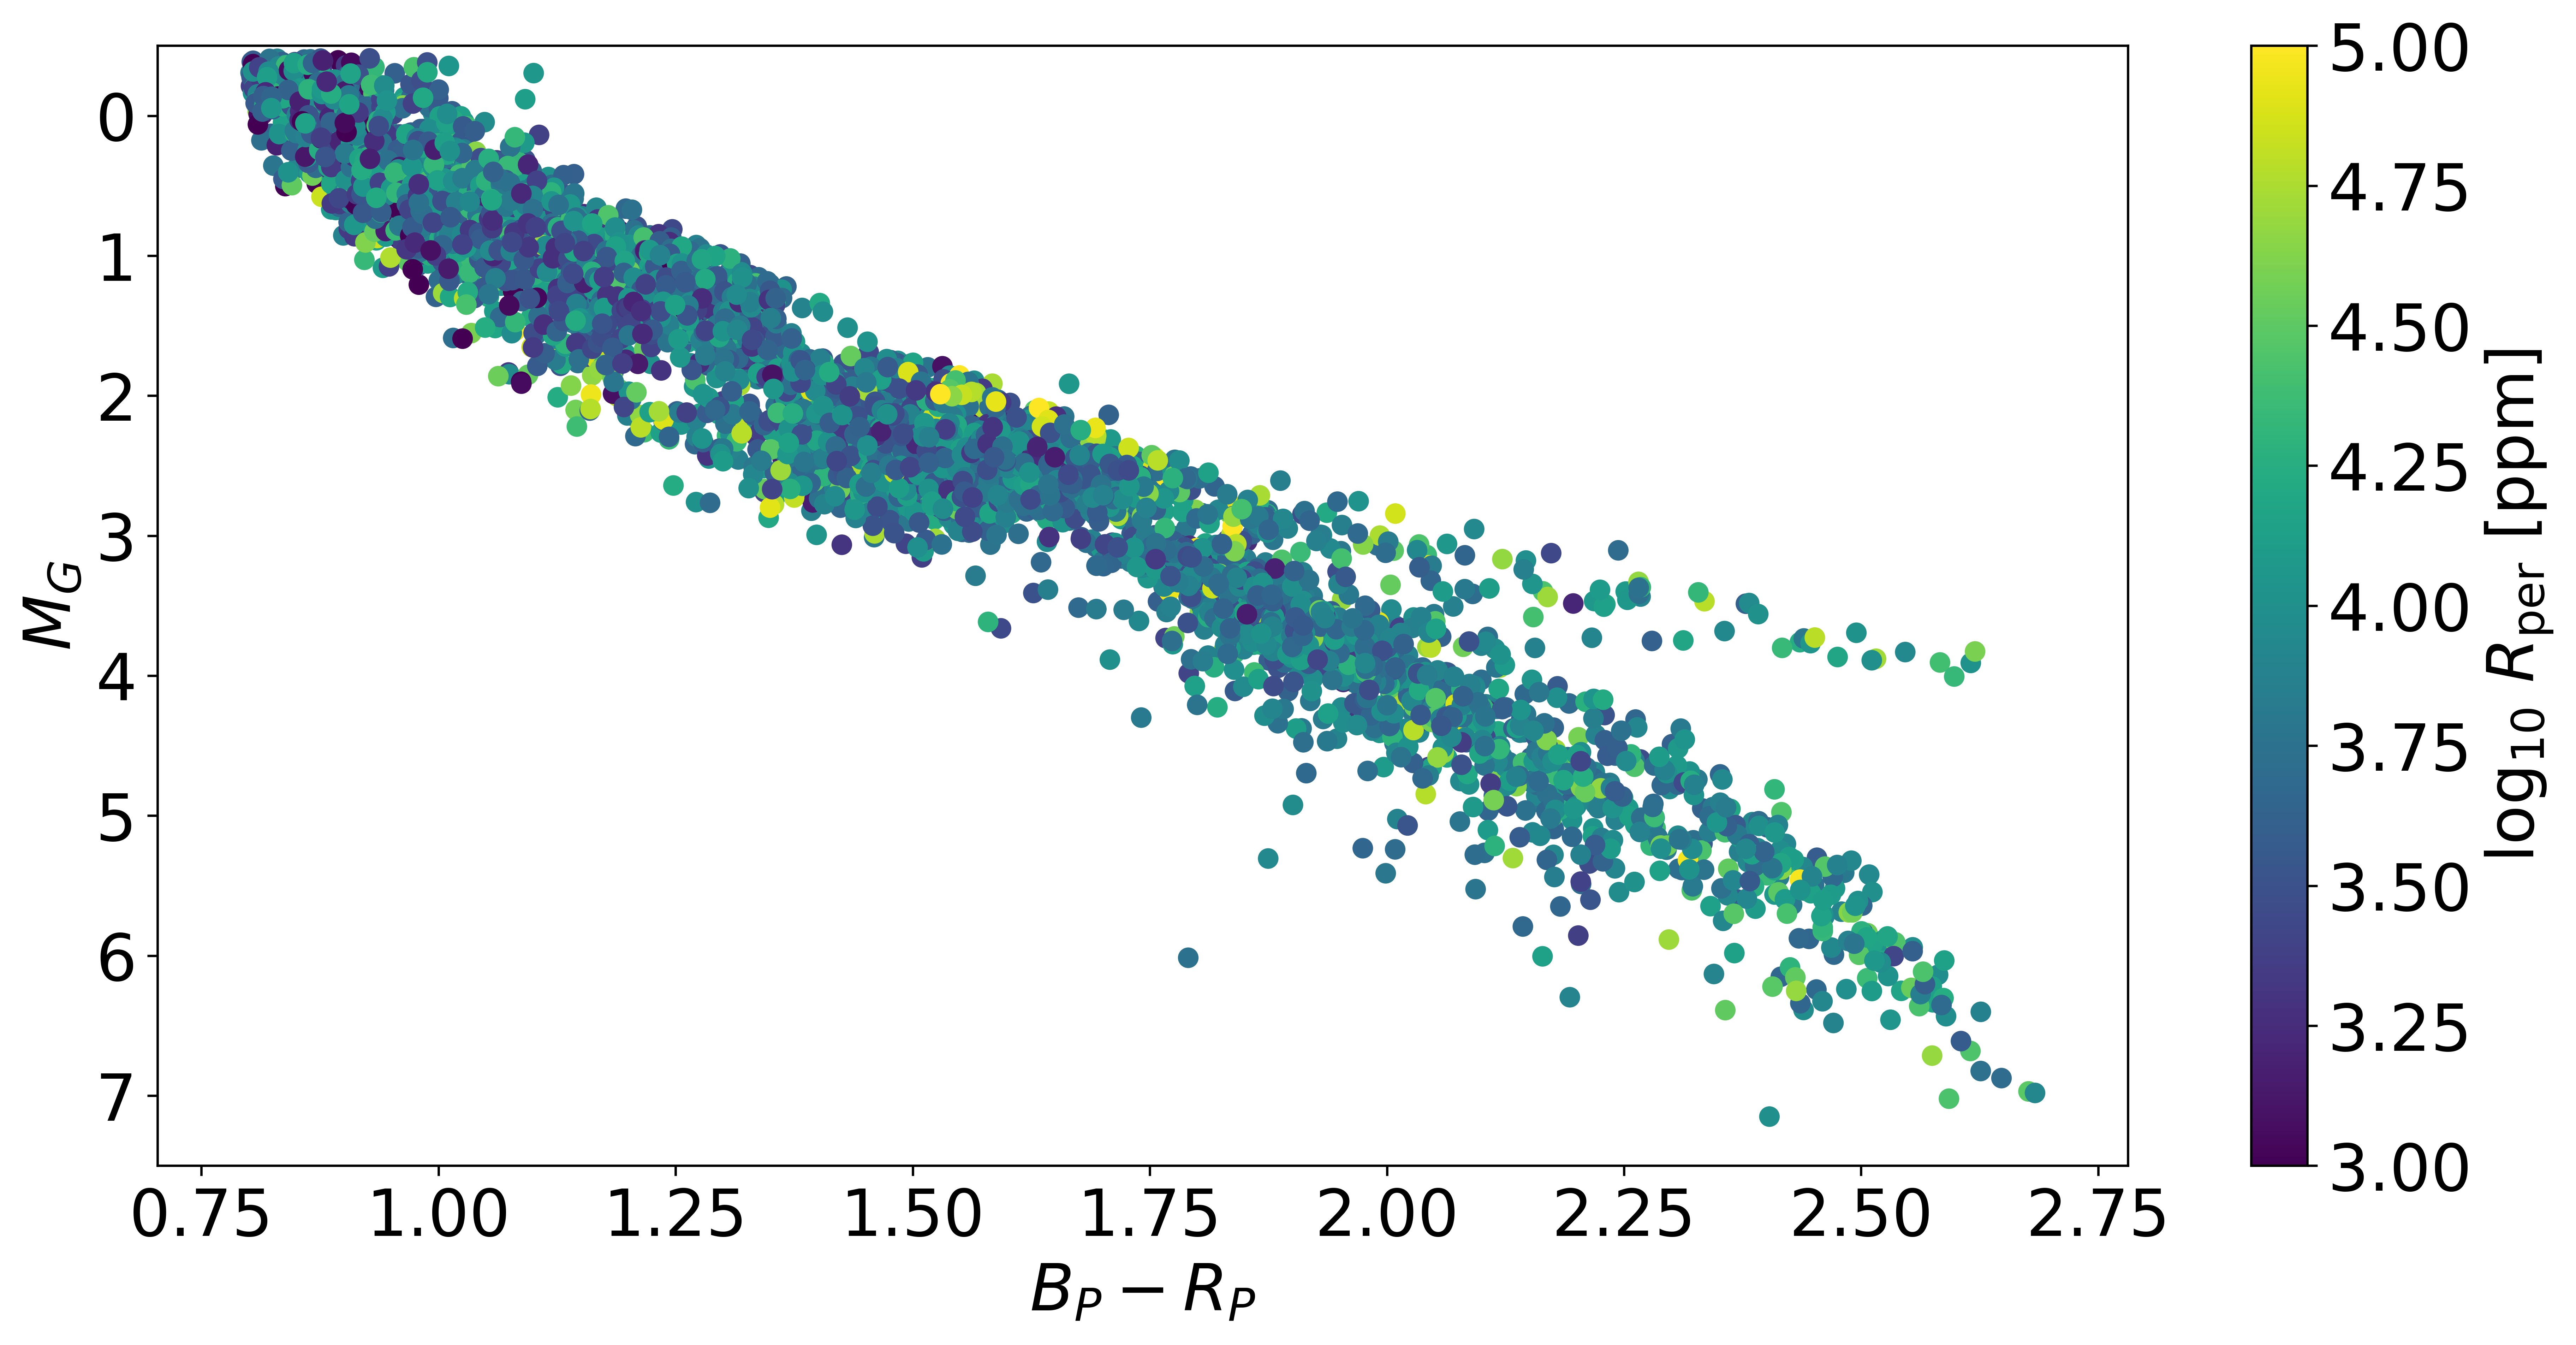
\includegraphics[width=\textwidth]{Figures/rot_gap_figures/HR.png}
    \caption{
    HR diagram of the closeby rotating main-sequence sample colours by photometric variability (\rper{}).}
    \label{fig:hr}
\end{figure}

\begin{figure}
\centering
    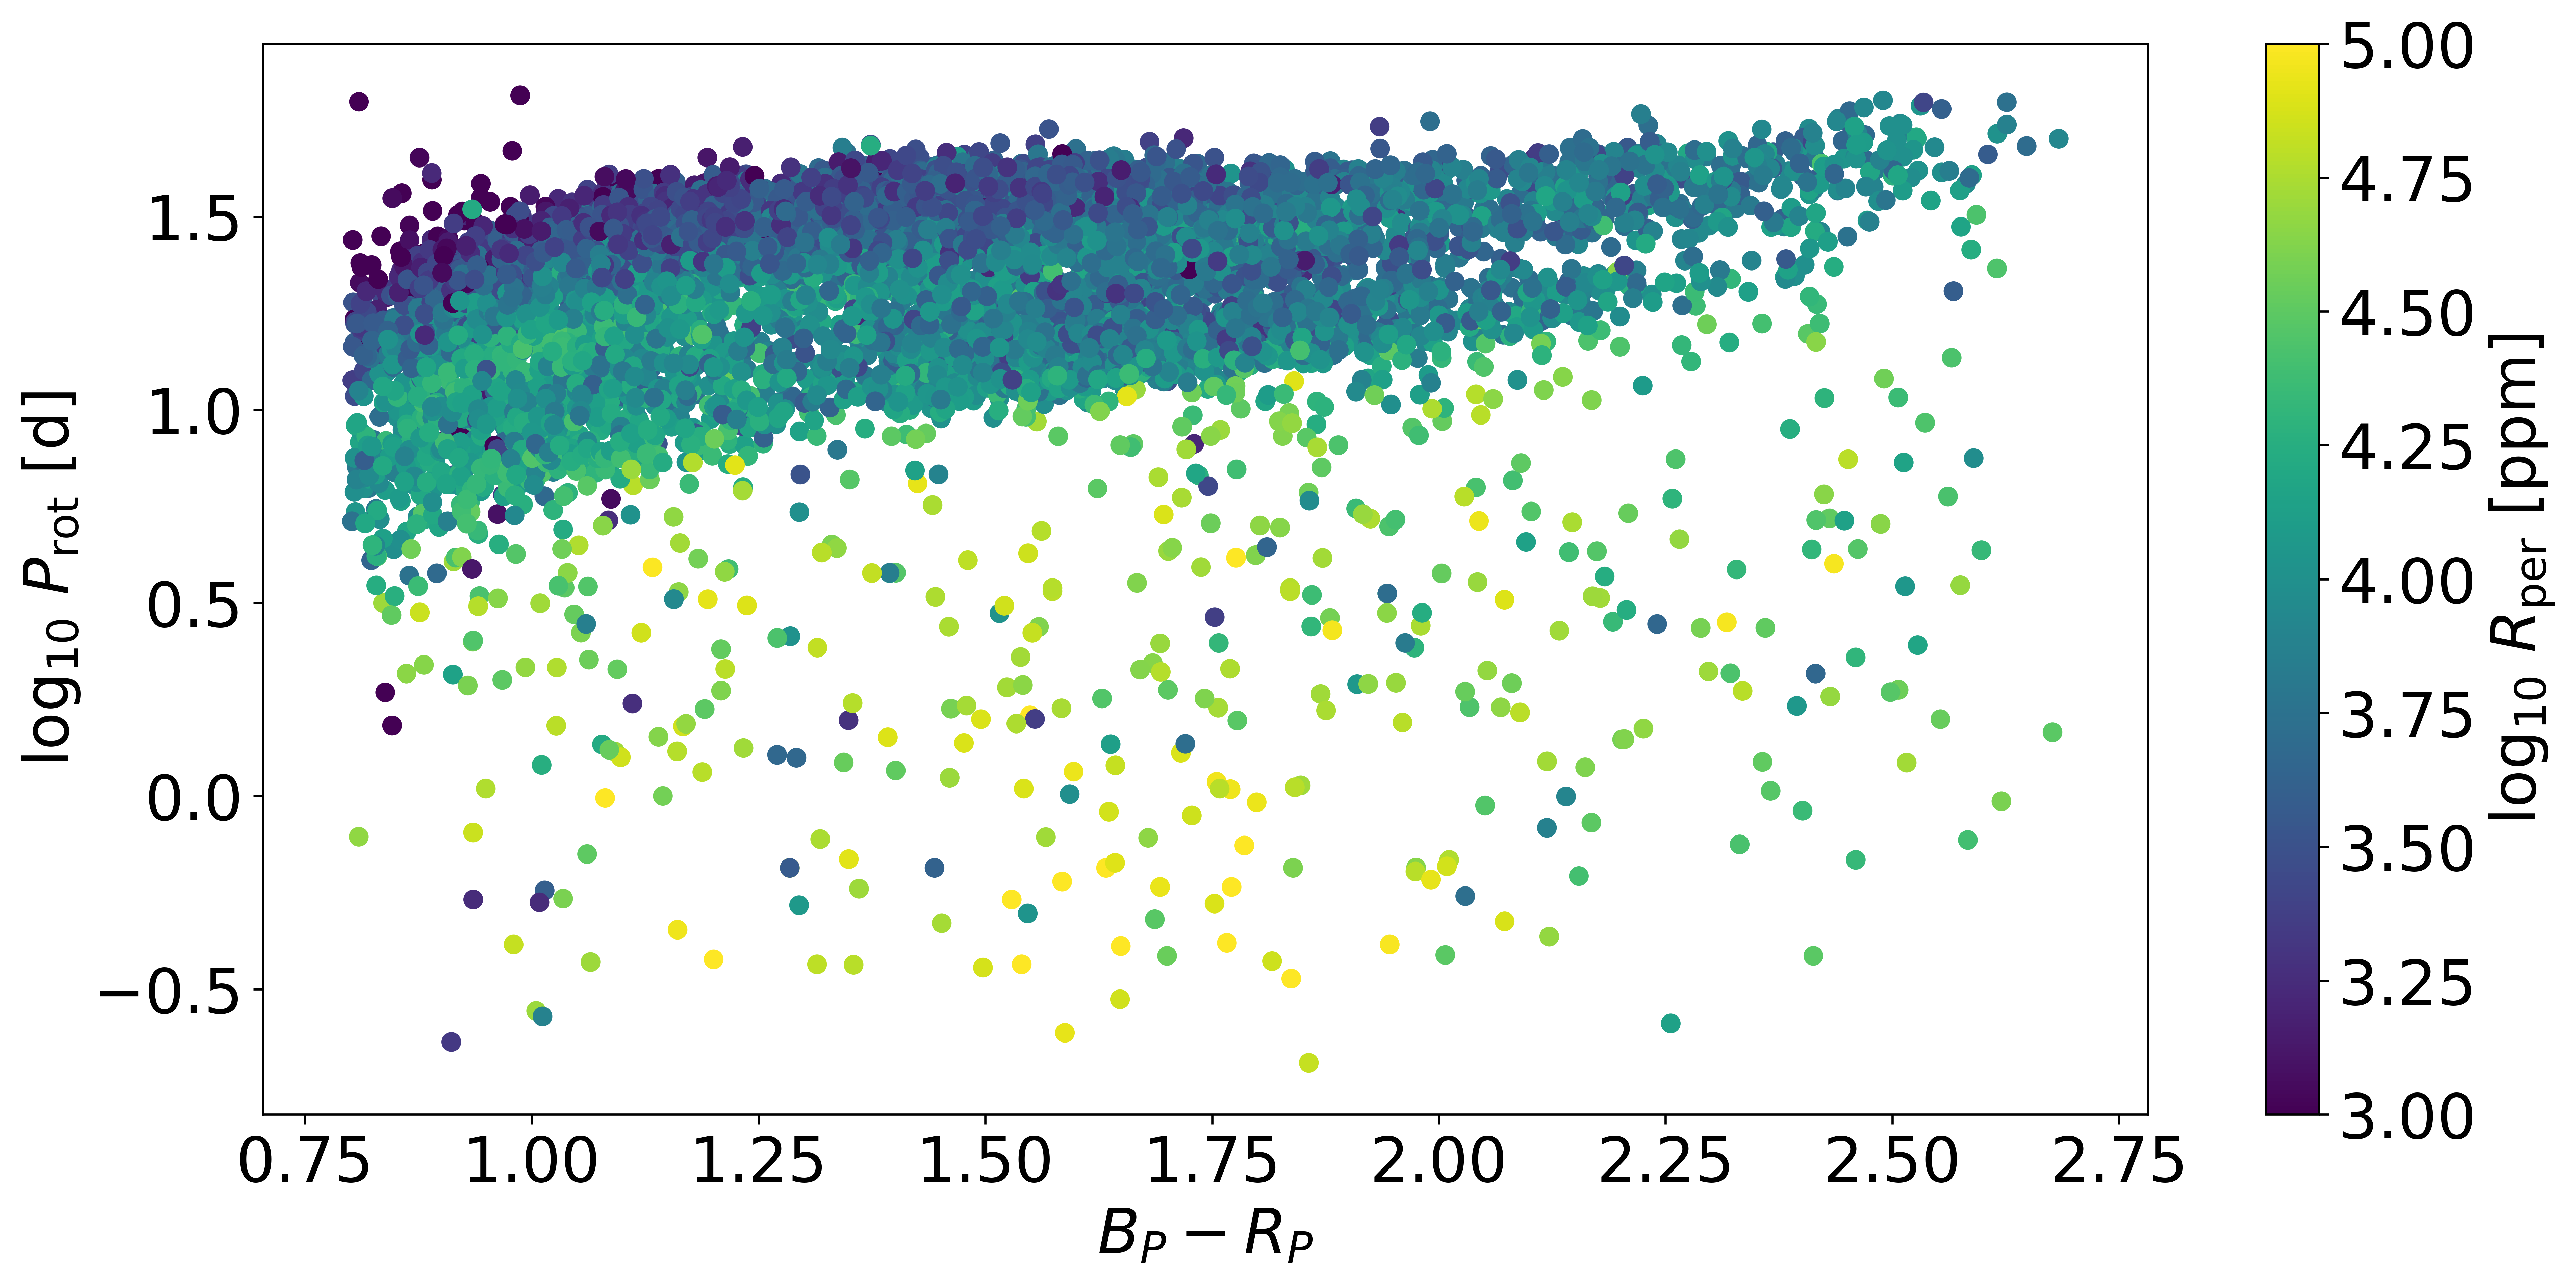
\includegraphics[width=\textwidth]{Figures/rot_gap_figures/rotational_dist.png}
    \caption{
    $\log_10$ of the rotation period against \gaia $B_P-R_P$ colour of the closeby rotating main-sequence sample colours by photometric variability (\rper{}). In this Figure we can see clearly see the decrease in photometric variability of stars near the gap.}
    \label{fig:prawn}
\end{figure}

From this sample we can establish a description of the average evolution of photometric variability around the intermediate period gap.
We will first separate the subsample into bins of $B_P - R_P$ (colour) from 0.8-2.5 of size 0.17 (10 bins).
In each colour interval, we then split the data into $log$ rotational period intervals of width 0.07 dex between 0.4 and 1.8 dex - which correspond to 2.5 and 70 days, respectively.
We then compute the median and median absolute deviation of \rper{} in each colour and rotational period bin.
The median is used here to attempt to alleviate the effect of activity cycles on the variance on the magnetic activity and the median absolute deviation establishes the scatter on the measured photometric variability - regions with large median absolute deviation should be treated as less reliable measurements.
We neglected the regions with few stars ($<$5).
This removes the spurious stars that have not ascended onto the lower prong of the intermediate period gap, which do not indicate large-scale trends in the data.
We reconfirm that \rper{} tends to increase with mass, decrease with the rotational period, and decrease towards the rotational period gap \citep{reinhold_stellar_2020, santos_surface_2021}.
Comparing Figures \ref{fig:prawn} and \ref{fig:binned_rper_full_sample}, we also confirm that the gap aligns itself with a minima in \rper{}.

\begin{figure}
\centering
    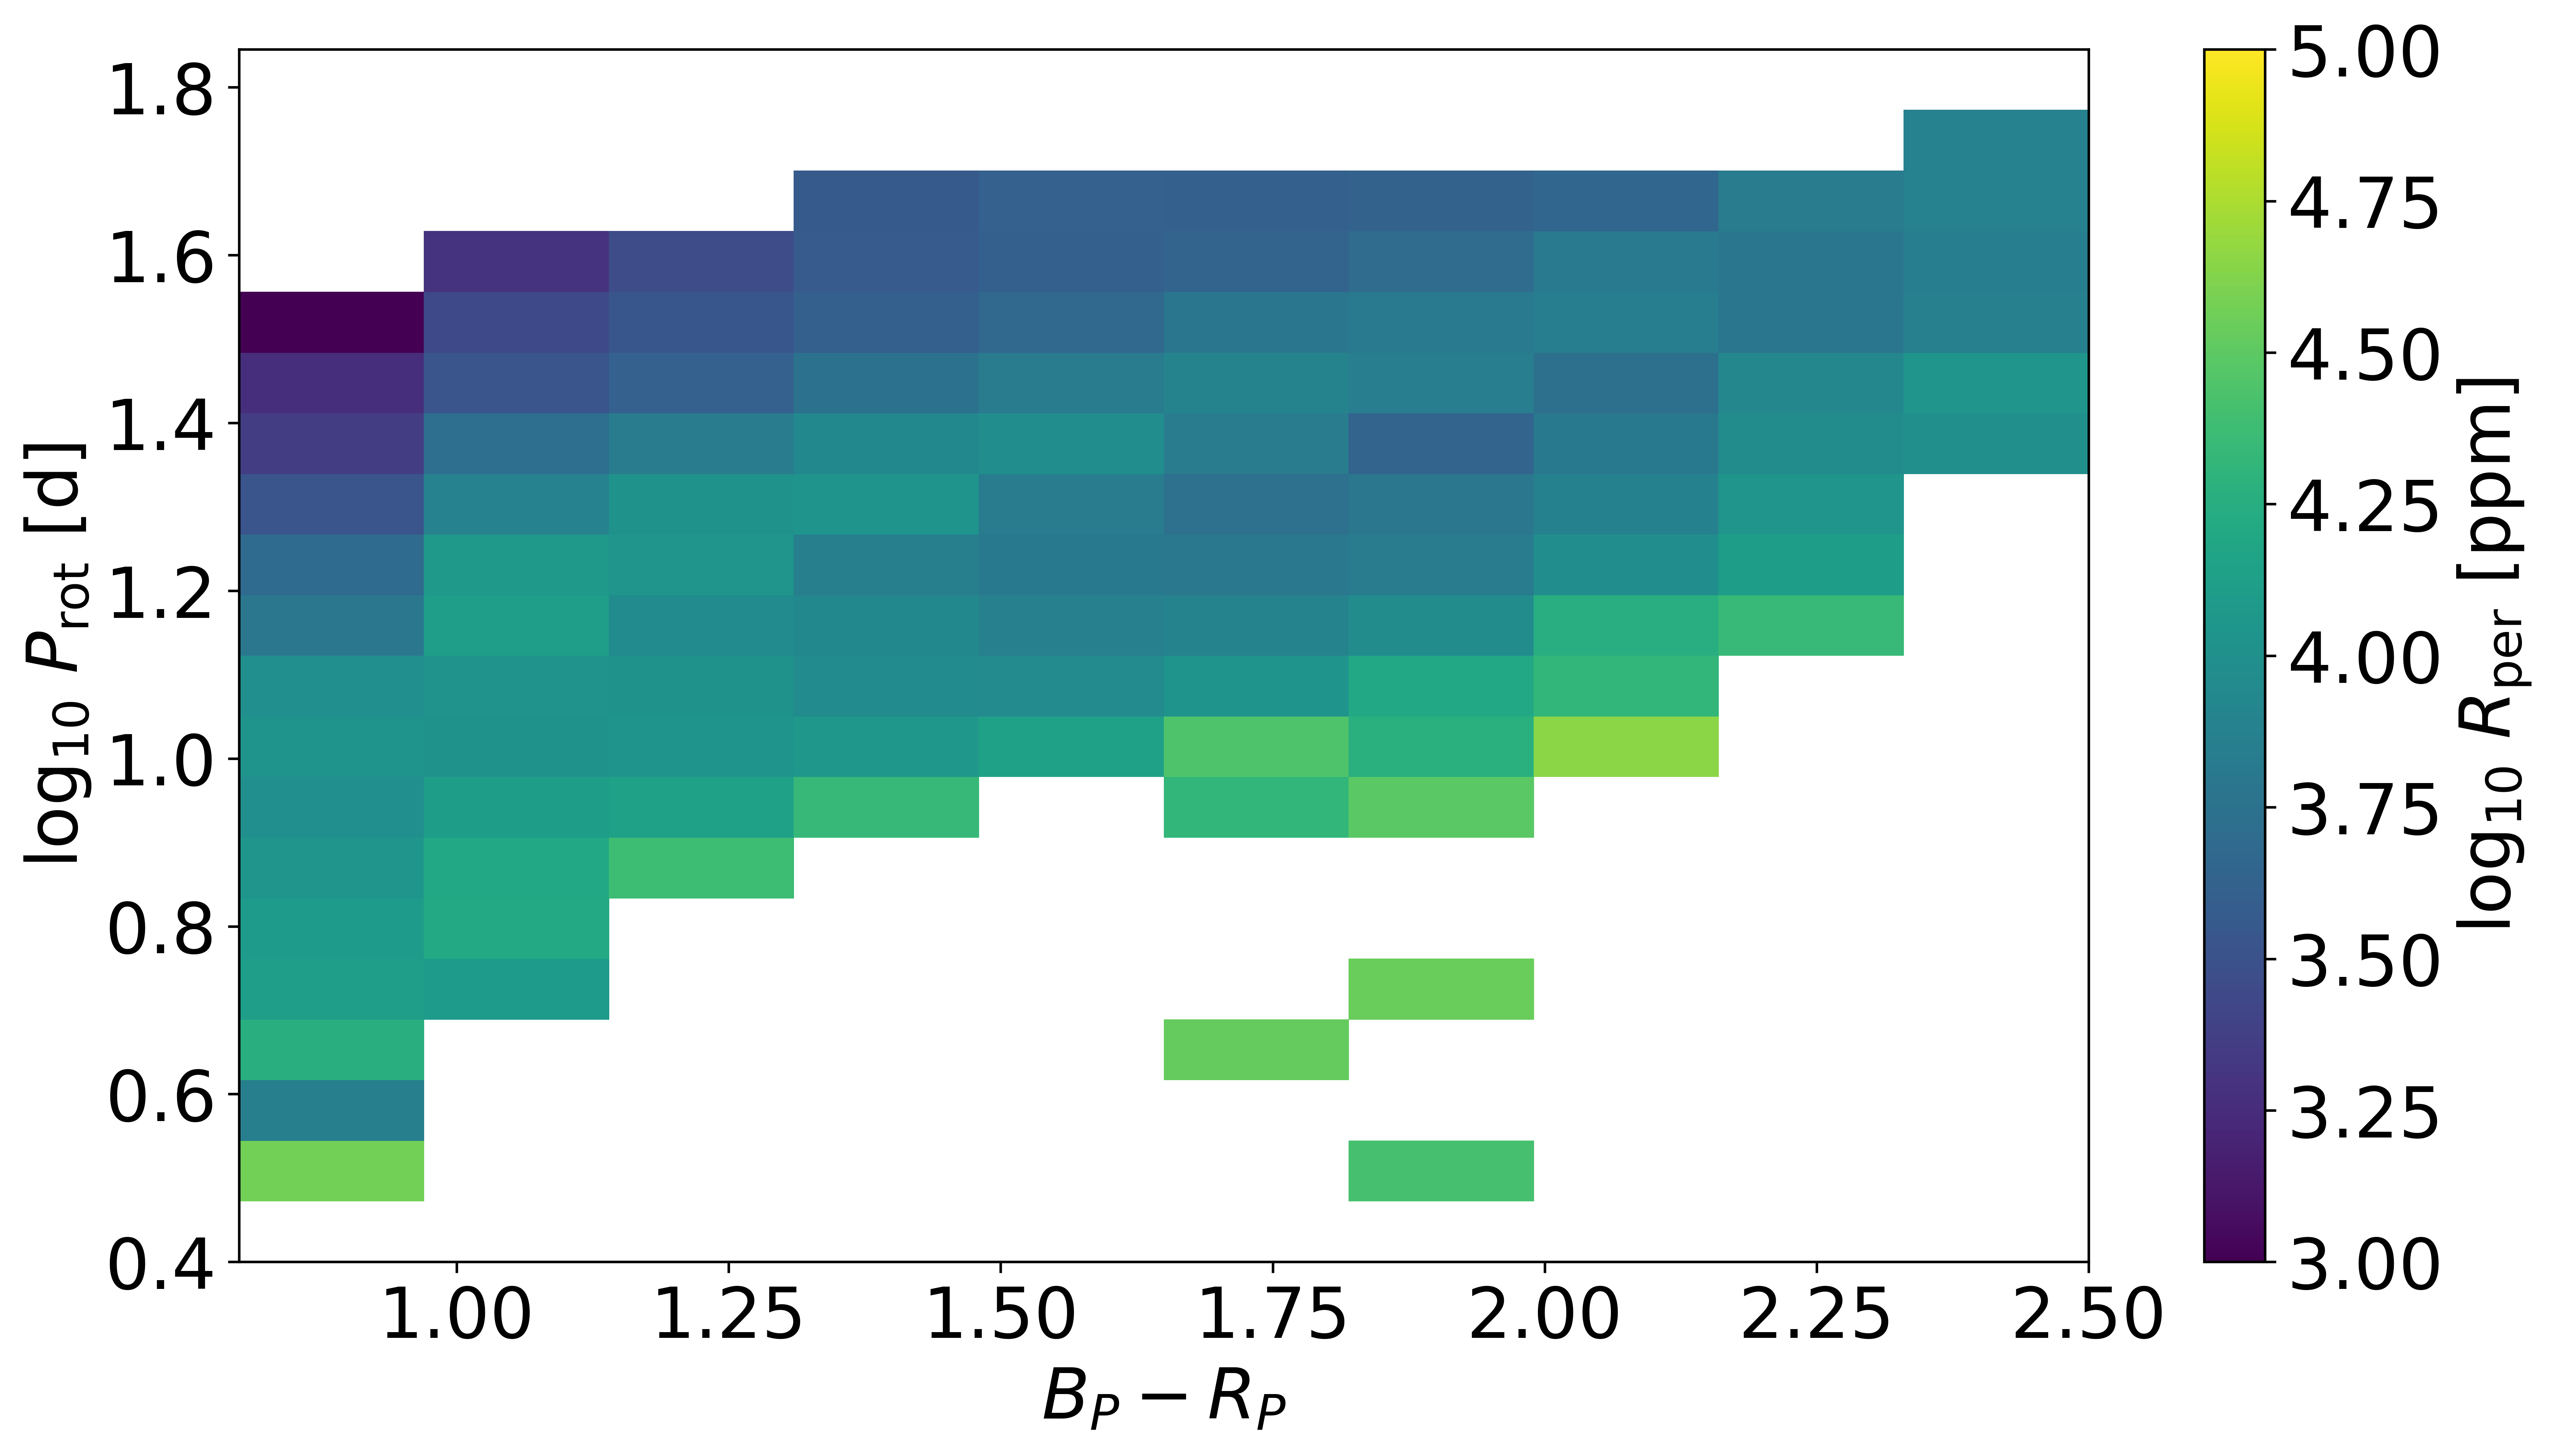
\includegraphics[width=\textwidth]{Figures/rot_gap_figures/rot_dist_binned.png}
    \caption{
    2D binned photometric variability (\rper{}) for the slices of $\log_10$ of the rotation period and colour \gaia $B_P-R_P$ used in this work. Comparing this Figure and \ref{fig:prawn} the alignment of the minima of photometric variability and observation of stars in the gap can be seen.}
    \label{fig:binned_rper_full_sample}
\end{figure}


As a result of the large-scale variability with stellar mass and rotational period, the position of the minima becomes harder to notice as $B_P - R_P$ approaches 0.8.
To make the minima more prominent, we plot the same data in Figure \ref{fig:binned_rper_scatter}.
We show the median \rper{} (scatter points) and scatter (errorbars) against the $\log_{10}$ of the rotation period for each colour range indicated in brackets - here, the colour of the interval increases down the plot - as well as fitted cubic spline to the data (dashed).
From the cubic spline, we can use the first and second derivatives of the spline to accurately determine the position of the local minima in \rper{}, which is indicated by the solid vertical blue line.
The calculation of the position of the minima is an automated process.
We first find where the first derivative is close to zero and where the second derivative is relatively large and greater than zero - this is to ensure we ignore any spurious jitter in the spline fit.
We use an automated process ensure we have not selected a position that we believe aligns with the intermediate period gap though the resulting position of minima can vary slightly depending on the smoothing of the cubic spline.
The first minima, in regards to the rotational period, in the $B_P-R_P$ (0.8-0.97) bin was manually ignored.
The position of the minima are shown in blue in Figure \ref{fig:indicating_minima}, where it is clear that the majority of minima align with the intermediate period gap.
We note that the minima do not accurately predict the position of the intermediate period gap for $B_P-R_P> 2.16$.
We believe this is because of the small number of stars below the gap in this colour range which were cut due to them not containing enough stars.
 With larger numbers of observations of low-mass stars below the gap we believe our prediction of the position of the rotation period gap with \rper{} \ would be more accurate in this regime. 
We also note that the average photometric modulation amplitude tends to peak to a maximum with a larger \rper{} than stars on the lower prong of the rotational period gap despite having longer rotation periods.
Whether this peak is indicative of stronger photometric activity suddenly above the gap or of suppression of photometric activity below the gap is unknown.

\begin{figure}
\centering
    \includegraphics[width=0.5\textwidth]{Figures/rot_gap_figures/rot_vs_rper_minima.png}
    \caption{
    Median and median absolute deviation of photometric variability (\rper{}) against $\log_10$ of the rotation period in bins of and colour \gaia{} $B_P-R_P$ (indicated in brackets). Here we have fitted a cubic spline to median \rper{} \ and calculated minima using the first and second derivatives of the fitted cubic spline. The minima here are shown by solid vertical blue lines. These minima align with the rotational period gap.}
    \label{fig:binned_rper_scatter}
\end{figure}

\begin{figure}
\centering
    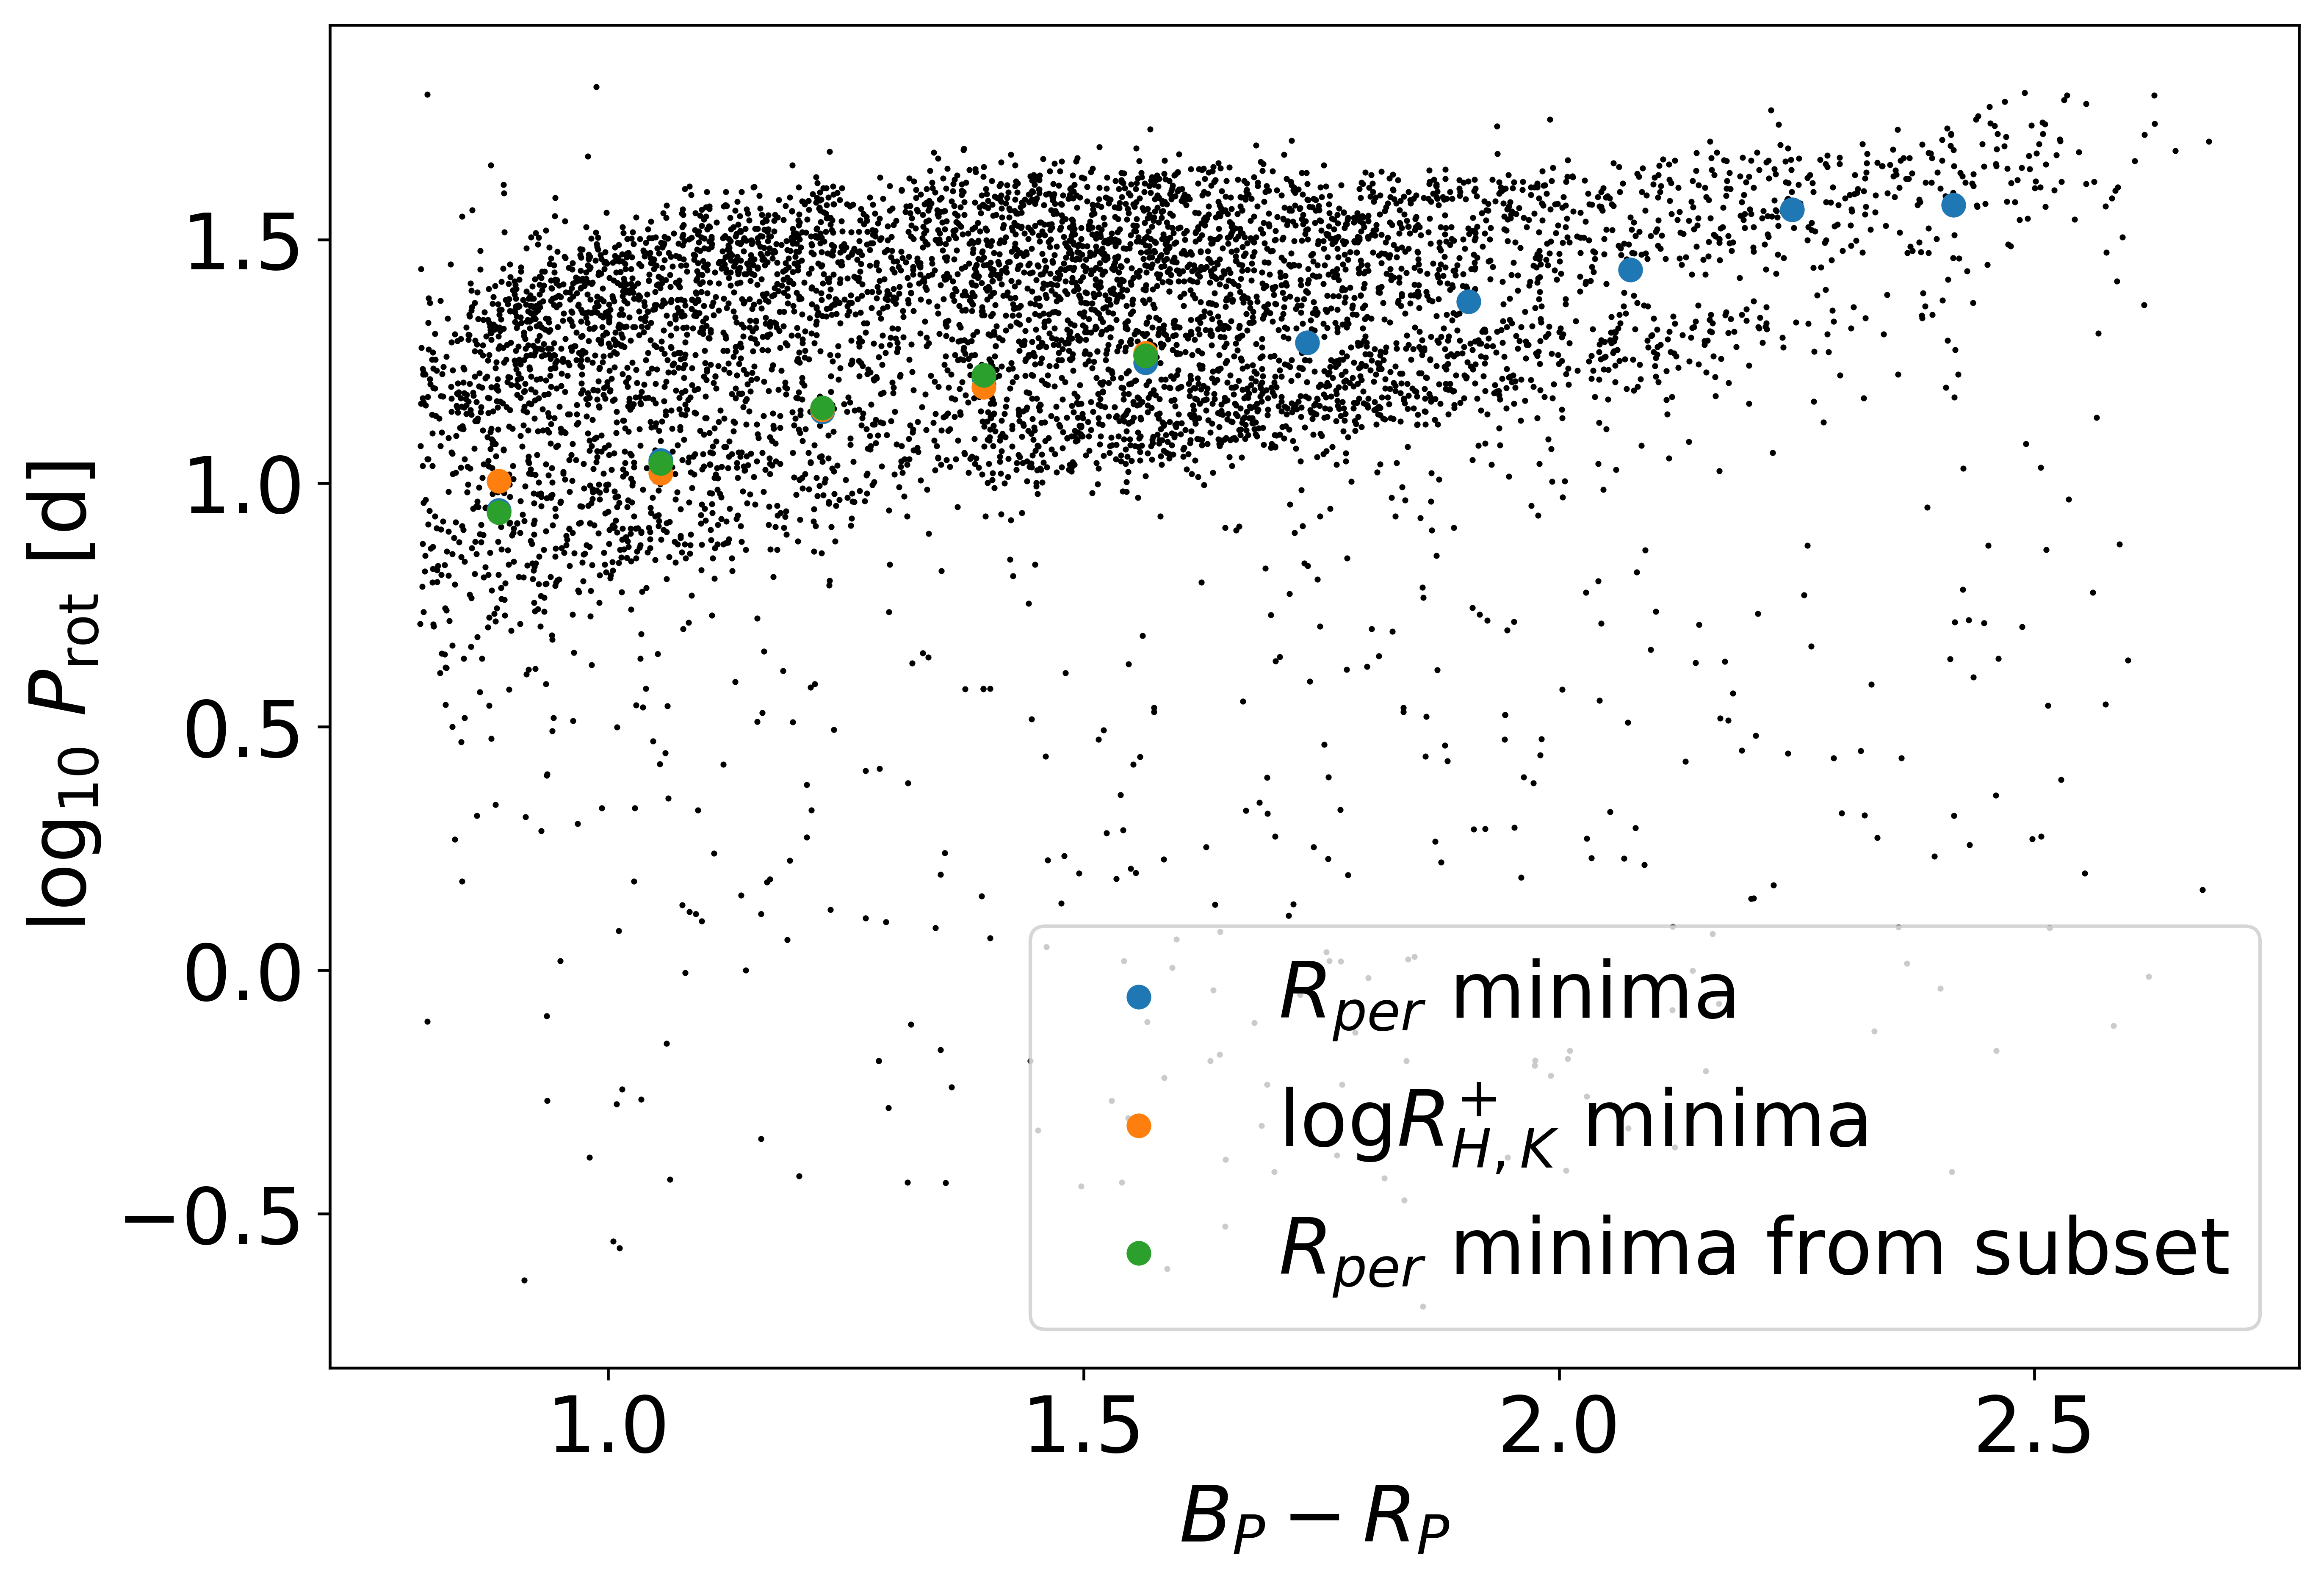
\includegraphics[width=\textwidth]{Figures/rot_gap_figures/rot_dist_minima_shown.png}
    \caption{
    The position of the identified minima in \rper{} \ against rotational period using the full close-by rotating main-sequence \kepler{} \ sample, the \rper{} minima identified with the \kepler{} LAMOST cross-match and the $\log_{10} R^{+}_{H,K}$ minima minima identified with the \kepler{} LAMOST cross-match.}
    \label{fig:indicating_minima}
\end{figure}

A possible explanation for the decrease in median photometric variability comes from the nature of the dearth of observations itself.
The gap is not horizontally aligned and increases in period for stars of lower mass (higher $B_P-R_P$).
\rper{} generally decreases with mass and rotation period.
Taking the median value in slices of constant rotation period near the dearth of observations will be systematically biased in different ways as it passes through the dearth.
In order of increasing rotation period, the slice will contain: (1) majority fast rotating but redder stars and a small number of slow-rotating bluer stars, (2) approximately equal fast-rotating red stars and slow-rotating blue stars, and finally (3) majority slow-rotating bluer stars and a small number of fast-rotating redder stars.
The relationship between the \rper{}, mass and rotation period are not easily parameterised - especially near the gap.
However, we can confirm that this effect does not skew our results by calculating the median and median absolute deviation of $B_P-R_P$ in each colour and rotational period bin.
We have shown this in Figure \ref{fig:colour_rper}.
We confirm that the minima and maxima of \rper{} with rotation period in each colour bin do not correspond to a minima or maxima in colour that would indicate that this effect is at play.
The variation is \rper{} is, therefore, a physical effect that aligns itself with the rotational period gap.

\begin{figure}
\centering
    \includegraphics[width=0.5\textwidth]{Figures/rot_gap_figures/per_vs_colour.png}
    \caption{
    Median and median absolute deviation of photometric variability (\rper{}) (blue) and $B_P-R_P$ (orange) against $\log_10$ of the rotation period in bins of and \gaia{} $B_P-R_P$ colour (indicated in brackets). The position of the minima in \rper{} \ do not align with a maxima or minima in $B_P-R_P$ implying that the colour bias when fitting across the dearth can be the cause of the \rper{} \ minima.}
    \label{fig:colour_rper}
\end{figure}


On first glance the minima in \rper{} surrounding the gap suggests that the rotation period gap is the result of the decreased probability to observe stars at the given rotation period.
However, the minima values of \rper{} within the gap can be otherwise be detected for other colour stars.
For example the minima in the $B_P-R_P$ - (0.97-1.14) slice has a \rper{} value of $\sim 4.0$ which can otherwise be easily detected for slower rotating or redder stars.
This either suggests that (a) the periodic variability drops suddenly to levels where rotation is not measureable at the rotation period gap or (b) the rotational variability drops as a result of the process by which stars cross the gap. 
 \citet{santos_surface_2021} increased the sensitivity of period detection for \kepler{} lightcurves and did not increase the number of stars observed near the intermediate period gap - suggesting that the drop in photometric variability does not result in a decreased probability to observe stars near the gap.
This implies that if the drop in photometric variability is not the cause for the dearth of observations near the rotational period gap and rather that the drop in photometric variability is purely coincident with the rotational period gap - suggesting that the mechanism underlying the two observations are one and the same.
\rper{} \ is not well defined for stars where rotation is not detected- as \rper{} is defined by the photometric variability range over the a rotational period time-scale.
Therefore we do not know whether the potential stars that lay within the gap, which we cannot observe because of the supposed dramatic decrease in \rper{}, do or do not suddenly decrease in \rper{}.

\section{The gap aligns with a minima in $\log R^{+}_{\rm{HK}}$ }
\label{sec:minima_rhk}

While it has been well established that the photometric variability of stars decreases towards the intermediate period gap other magnetic activity indicators have not been explored in this regard only the large-scale trends with stellar mass and rotation \citep{zhang_magnetic_2020}.
Suppose other magnetic activity indicators vary in the same fashion as \rper{} - decreasing to a minima at the rotational period gap. 
In that case, it is more likely that the decrease in \rper{} towards the gap results from a variation in the magnetic field of stars.
We will begin by testing whether this is indeed the case.

\citet{zhang_magnetic_2020} extracted the chromospheric magnetic activity indexes, S and $\log \ R^{+}_{HK}$, for 59,816 stars from low-resolution LAMOST spectra in the LAMOST-Kepler program.
The cross-match of their work with the nearby rotating main sequence we established yielded 1060 stars.
The stars in the cross-match tend to be the higher mass, brighter, stars with $B_P-R_P<1.8$, where the intermediate period gap is less apparent.
Given that we could predict the position of the gap for these stars in our earlier experiment, we carry forward and re-analyse their data under a new framework.

$\log \ R^{+}_{HK}$ provides a more accurate measure of the chromospheric magnetic activity than $S$, which is uncoupled from a radiative contribution, so we adopt $\log \ R^{+}_{HK}$ in this work.
The resulting rotational distribution of stars are shown in Figure \ref{fig:rot_dist_rhk} coloured by $\log \ R^{+}_{HK}$.
Due to the smaller number of stars and lower precision of $\log \ R^{+}_{HK}$ than \rper{} it is not clear whether $\log \ R^{+}_{HK}$, like \rper{} decreases towards to the intermediate period gap.


\begin{figure}
\centering
    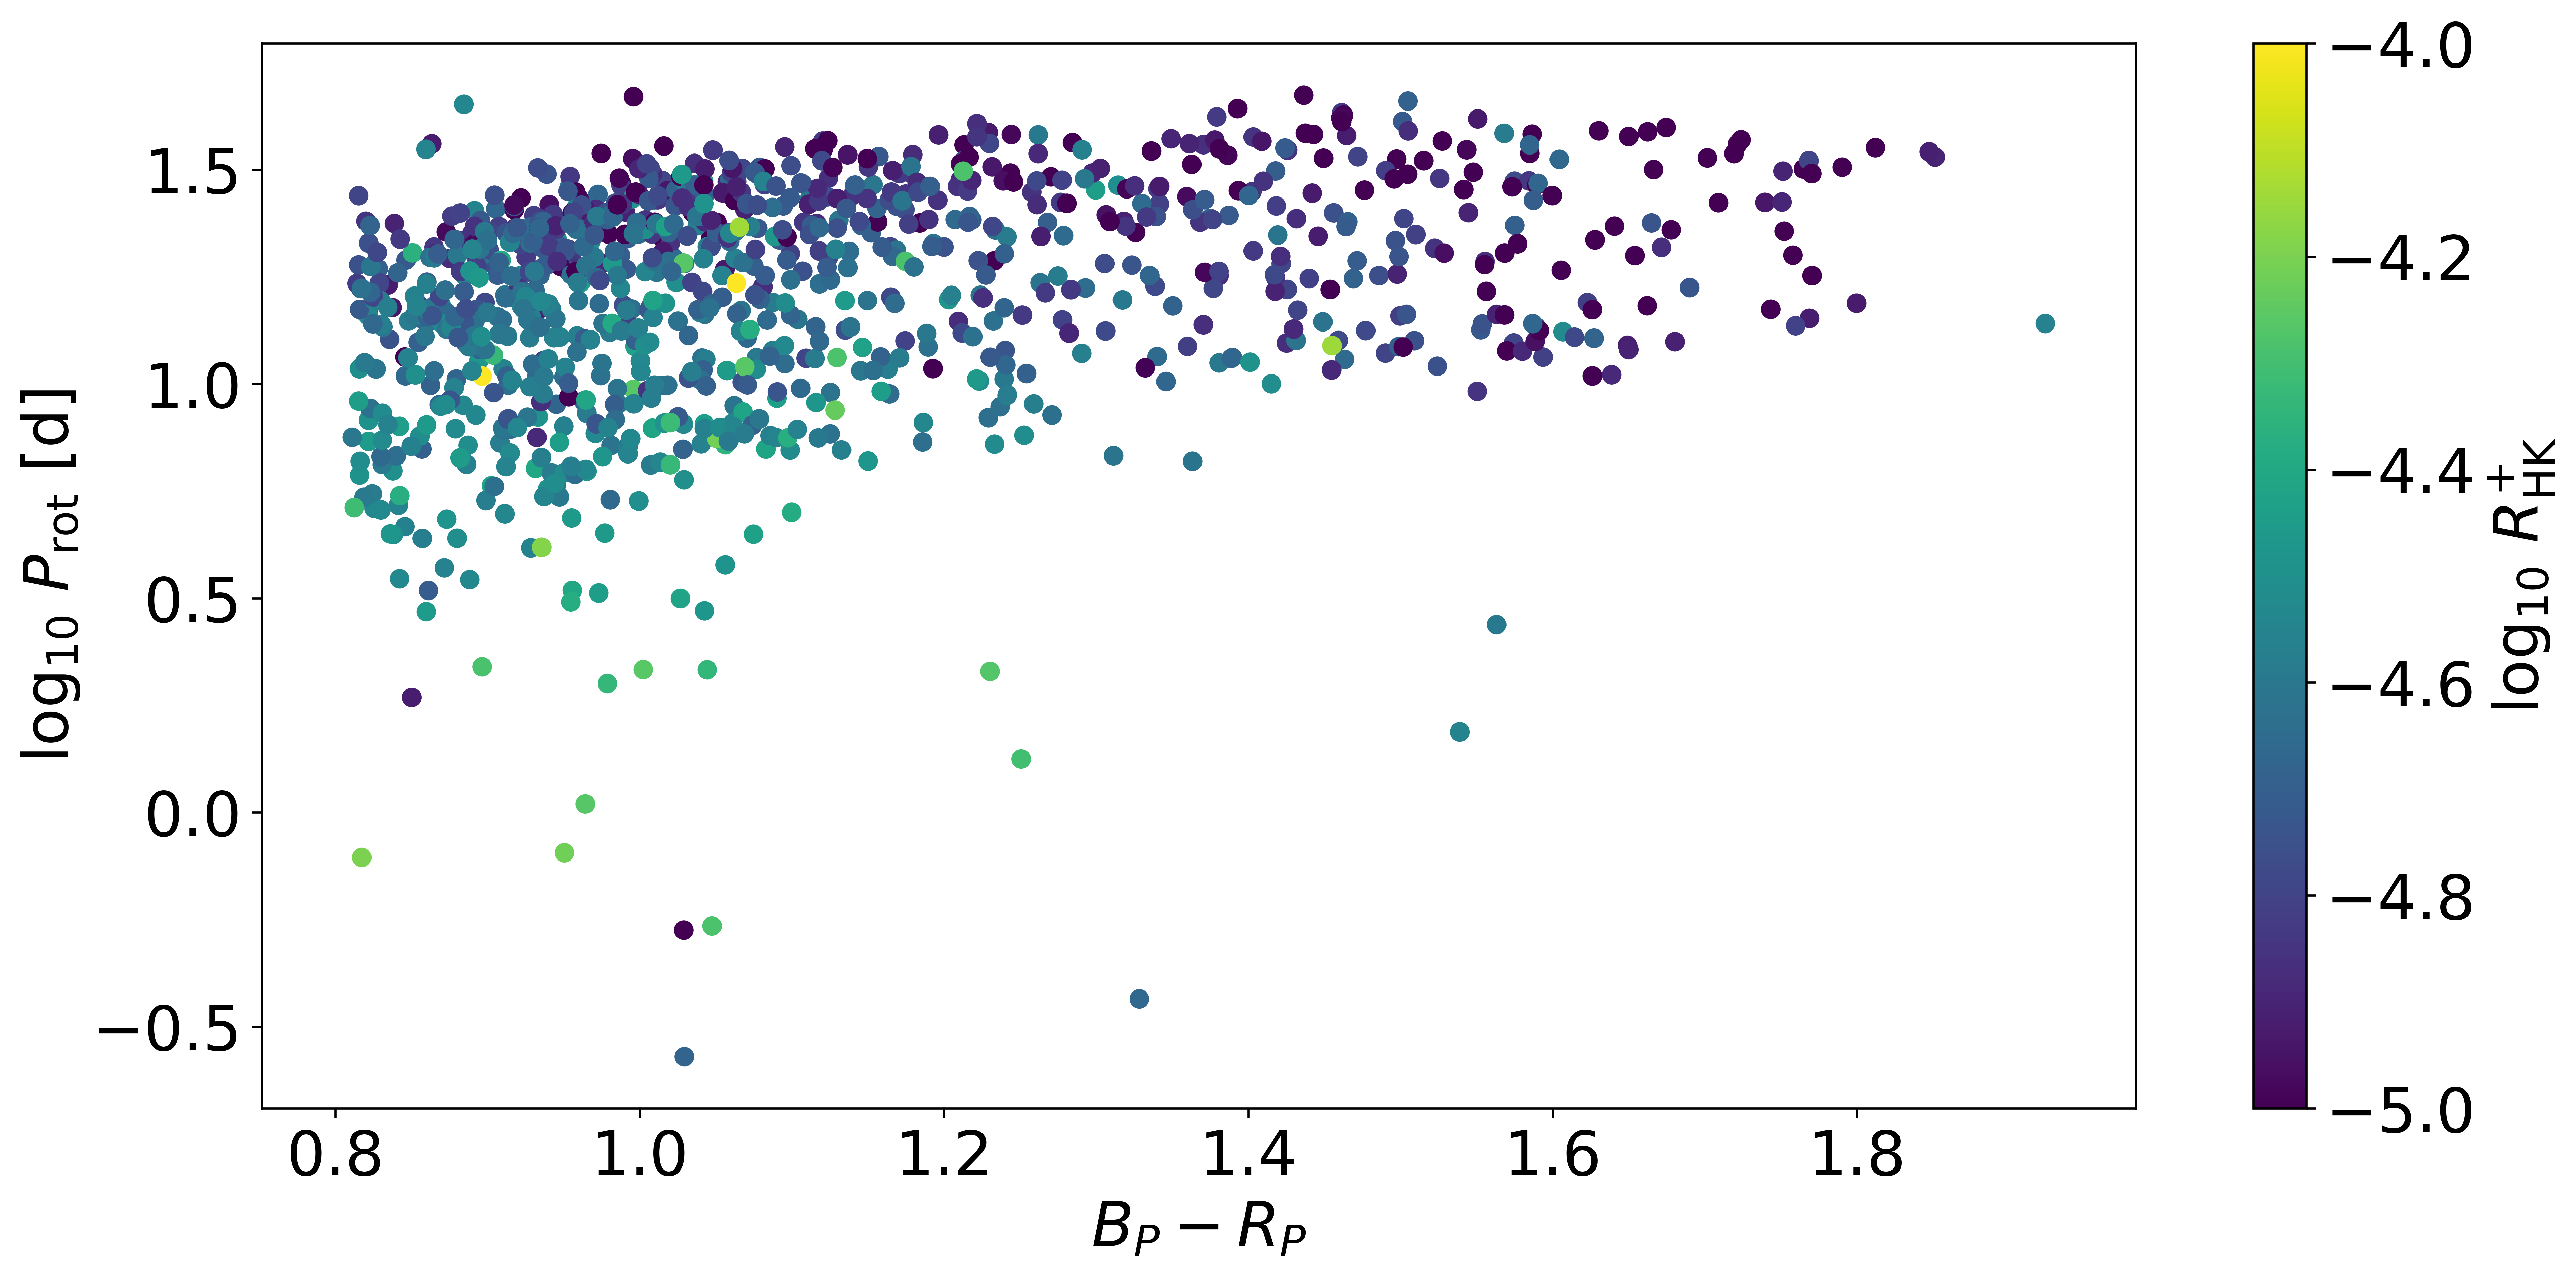
\includegraphics[width=\textwidth]{Figures/rot_gap_figures/rotational_dist_rhk.png}
    \caption{
    The LAMOST chromospherically active and \kepler{} rotating closeby, main-sequence cross-match $\log_{10}$ of rotational period $\log_10$ against \gaia $B_P-R_P$ colour coloured by $\log_{10}R^{+}_{\rm{HK}}$. It is unclear from this whether $\log_{10}R^{+}_{\rm{HK}}$ decreases toward the gap like \rper{}.}
    \label{fig:rot_dist_rhk}
\end{figure}

To determine this more concretely, we adopt the same process as we described earlier to find the minima in \rper{} \ in a bin of colour against the rotational period.
We again separate the stars into the same slices of $B_P-R_P$ and log of rotation period and remove any bins containing small numbers of stars ($<$2).
This cut-off was chosen because of the reduced number of stars in the sample but the results should therefore be treated with more caution because we are relying on small number statistics.
The median and median absolute deviation of both $\log \ R^{+}_{HK}$ and \rper{} \ in these slices was then calculated, which we then fit with cubic splines against the log of rotation period.
We have repeated this method on \rper{} \ here because we are using a subset of the original stars and to compare the recovered minima from the subset more accurately - this also allows us to confirm the accuracy of the fit of our minima in the first test.
The minima of the cubic spline fits are then calculated again using the first and second derivatives.

\begin{figure}
\centering
    \includegraphics[width=0.5\textwidth]{Figures/rot_gap_figures/rot_vs_rper_rhk_minima.png}
    \caption{
    Median and median absolute deviation of photometric variability (\rper{}) (blue) and LAMOST $\log_{10}R^{+}_{\rm{HK}}$ against $\log_10$ of the rotation period in bins of and colour \gaia{} $B_P-R_P$ (indicated in brackets). Here we have fitted a cubic spline to median of these values in each bin and calculated minima using the first and second derivatives of the fitted cubic spline. The minima in \rper{} are shown by solid vertical blue lines while the minima in $\log_{10}R^{+}_{\rm{HK}}$ are shown in solid vertical orange lines. These minima align with each other and the rotational period gap.}
    \label{fig:rot_rper_rhk}
\end{figure}

We compare the distributions of \rper{} \ and $\log \ R^{+}_{HK}$ against the log of rotation period in Figure \ref{fig:rot_rper_rhk} and show the found minima in blue and orange solid vertical lines for \rper{} \ and $\log \ R^{+}_{HK}$ respectively.
Like photometric variability, $\log \ R^{+}_{HK}$ tends to decrease with rotational period - owing to their relation to the strength of the magnetic field.
We find that, generally, \rper{} \ and $\log \ R^{+}_{HK}$ are directly tied - increases and decreases to the median value with rotational period in one tends to align with a similar response in the other.

We show the comparison of the recovered minima from \rper{} using this subset as well as the minima recovered using $\log \ R^{+}_{HK}$ in Figure \ref{fig:indicating_minima}.
The recovered \rper{} \ minima using the subset lay on top of the \rper{} minima recovered using the full sample.
Interestingly, we may detect previously unreported minima in $\log \ R^{+}_{HK}$ close to the rotation period gap.
Excluding the minima recovered in the $B_P-R_P$ - (0.8-0.97) bins, the minima that we recover in $\log \ R^{+}_{HK}$ against logged rotational period are in the same period bin and are close in position to the minima of \rper{} we recover, which we have established aligns with the intermediate period gap.
The alignment of the minima is also robust to variation in the smoothness of the fitted cubic spline - suggesting that the minima are not spurious.


Measurements of $\log \ R^{+}_{HK}$ are less precise than \rper{}, which is reflected in the relatively larger median absolute deviation.
The detection of the coincidence in a single slice of $B_P-R_P$ could be explained through this imprecision.
However, the detection of this in multiple slices of $B_P-R_P$ suggests that the cause of the minima is related.
Further study of this relationship is required to confirm the coincidence of the minima with a larger dataset of chromospheric magnetic activity indicators or with other magnetic activity indicators.
We will assume for now that the rotational period gap does align itself with minima in both \rper{} and $\log \ R^{+}_{HK}$ and explore whether there is a sample of low-magnetic activity, non-detected rotators. 

\section{Do we observe a sample of low-magnetic activity gap stars?}
\label{sec:low_activity_gap}

If the gap contains stars that have dramatically low \rper{} and thus do not have detectable rotation periods, then $\log \ R^{+}_{HK}$ should also dramatically drop within this region.
Further, if there is a sample of dramatically lower $\log \ R^{+}_{HK}$ stars without detected rotation periods then this sample supports the hypothesis that the intermediate period gap is the result of a decreased probability to observe stars at those rotation periods due to a decrease in stellar activity.
However, we do not know if stars without detected rotation periods align with the gap nor do we have a way to predict the expected spuriously low $\log \ R^{+}_{HK}$ values that would be required to explain the rotational period gap.
On the other hand, consider the relation between the detectability of rotation period, the magnetic activity indicators, and colour.
If, for example, there is a consistent region in ultra low-magnetic activity, below the expected range from the decrease in magnetic activity with stellar age, and colour space where rotational detectability is low, then this suggests that the rotational period gap arises from a sudden drop in magnetic activity and thus a drop in rotational detectability.

We will compare the $\log \ R^{+}_{HK}$  distributions of the \citet{mcquillan_rotation_2014} rotating and non-rotating samples.
To determine whether a star has a significant rotational period detection \citet{mcquillan_rotation_2014} defines a weight of the significance of the detection of the rotational period $w$ and compares this to a threshold value.
$w$ is defined in terms of the ACF's local peak height (LPH), the height of the selected peak with respect to the mean of the troughs on either side, the star's temperature and the rotational period.
For a more thorough description of their method for calculating this value see Section A in the appendix of their work.
This normalised value is calculated for each star and compared to a threshold value.
Those that do not pass the threshold were placed into a separate category of stars that do not have a detectable rotation period \footnote{ This is a slight misnomer as \textit{some} of the stars $\sim$ 100,000 stars have detectable rotation periods, but those periods should be treated with some care.}.

We prepare the sample of 99,000 non-rotating stars from their work in the same way that we did for the rotating sample - ensuring they are close by ($<525 pc$), on the main-sequence and redder than $B_P-R_P$  = 0.8 where the rotational period gap is most apparent.
This leaves us with a sample of 5574 non-rotating close by, main-sequence stars which we can cross match with the LAMOST-\kepler{} \ sample of chromospheric active stars measured in \citet{zhang_magnetic_2020} - reducing the number of stars to 1134 stars.
The number of stars in this sample is similar to the number of stars in the rotating sample.
We show the resulting HR diagram of stars without rotational detection (bottom) and with rotational detection (top) in Figure \ref{fig:non_rotating_mag_hr} coloured by $\log \ R^{+}_{HK}$.
Comparing the distributions it is clear that the non-rotating sample is clearly biased for higher mass stars and does not permeate into the low mass regime, where the gap would be most apparent.


\begin{figure}
\centering
    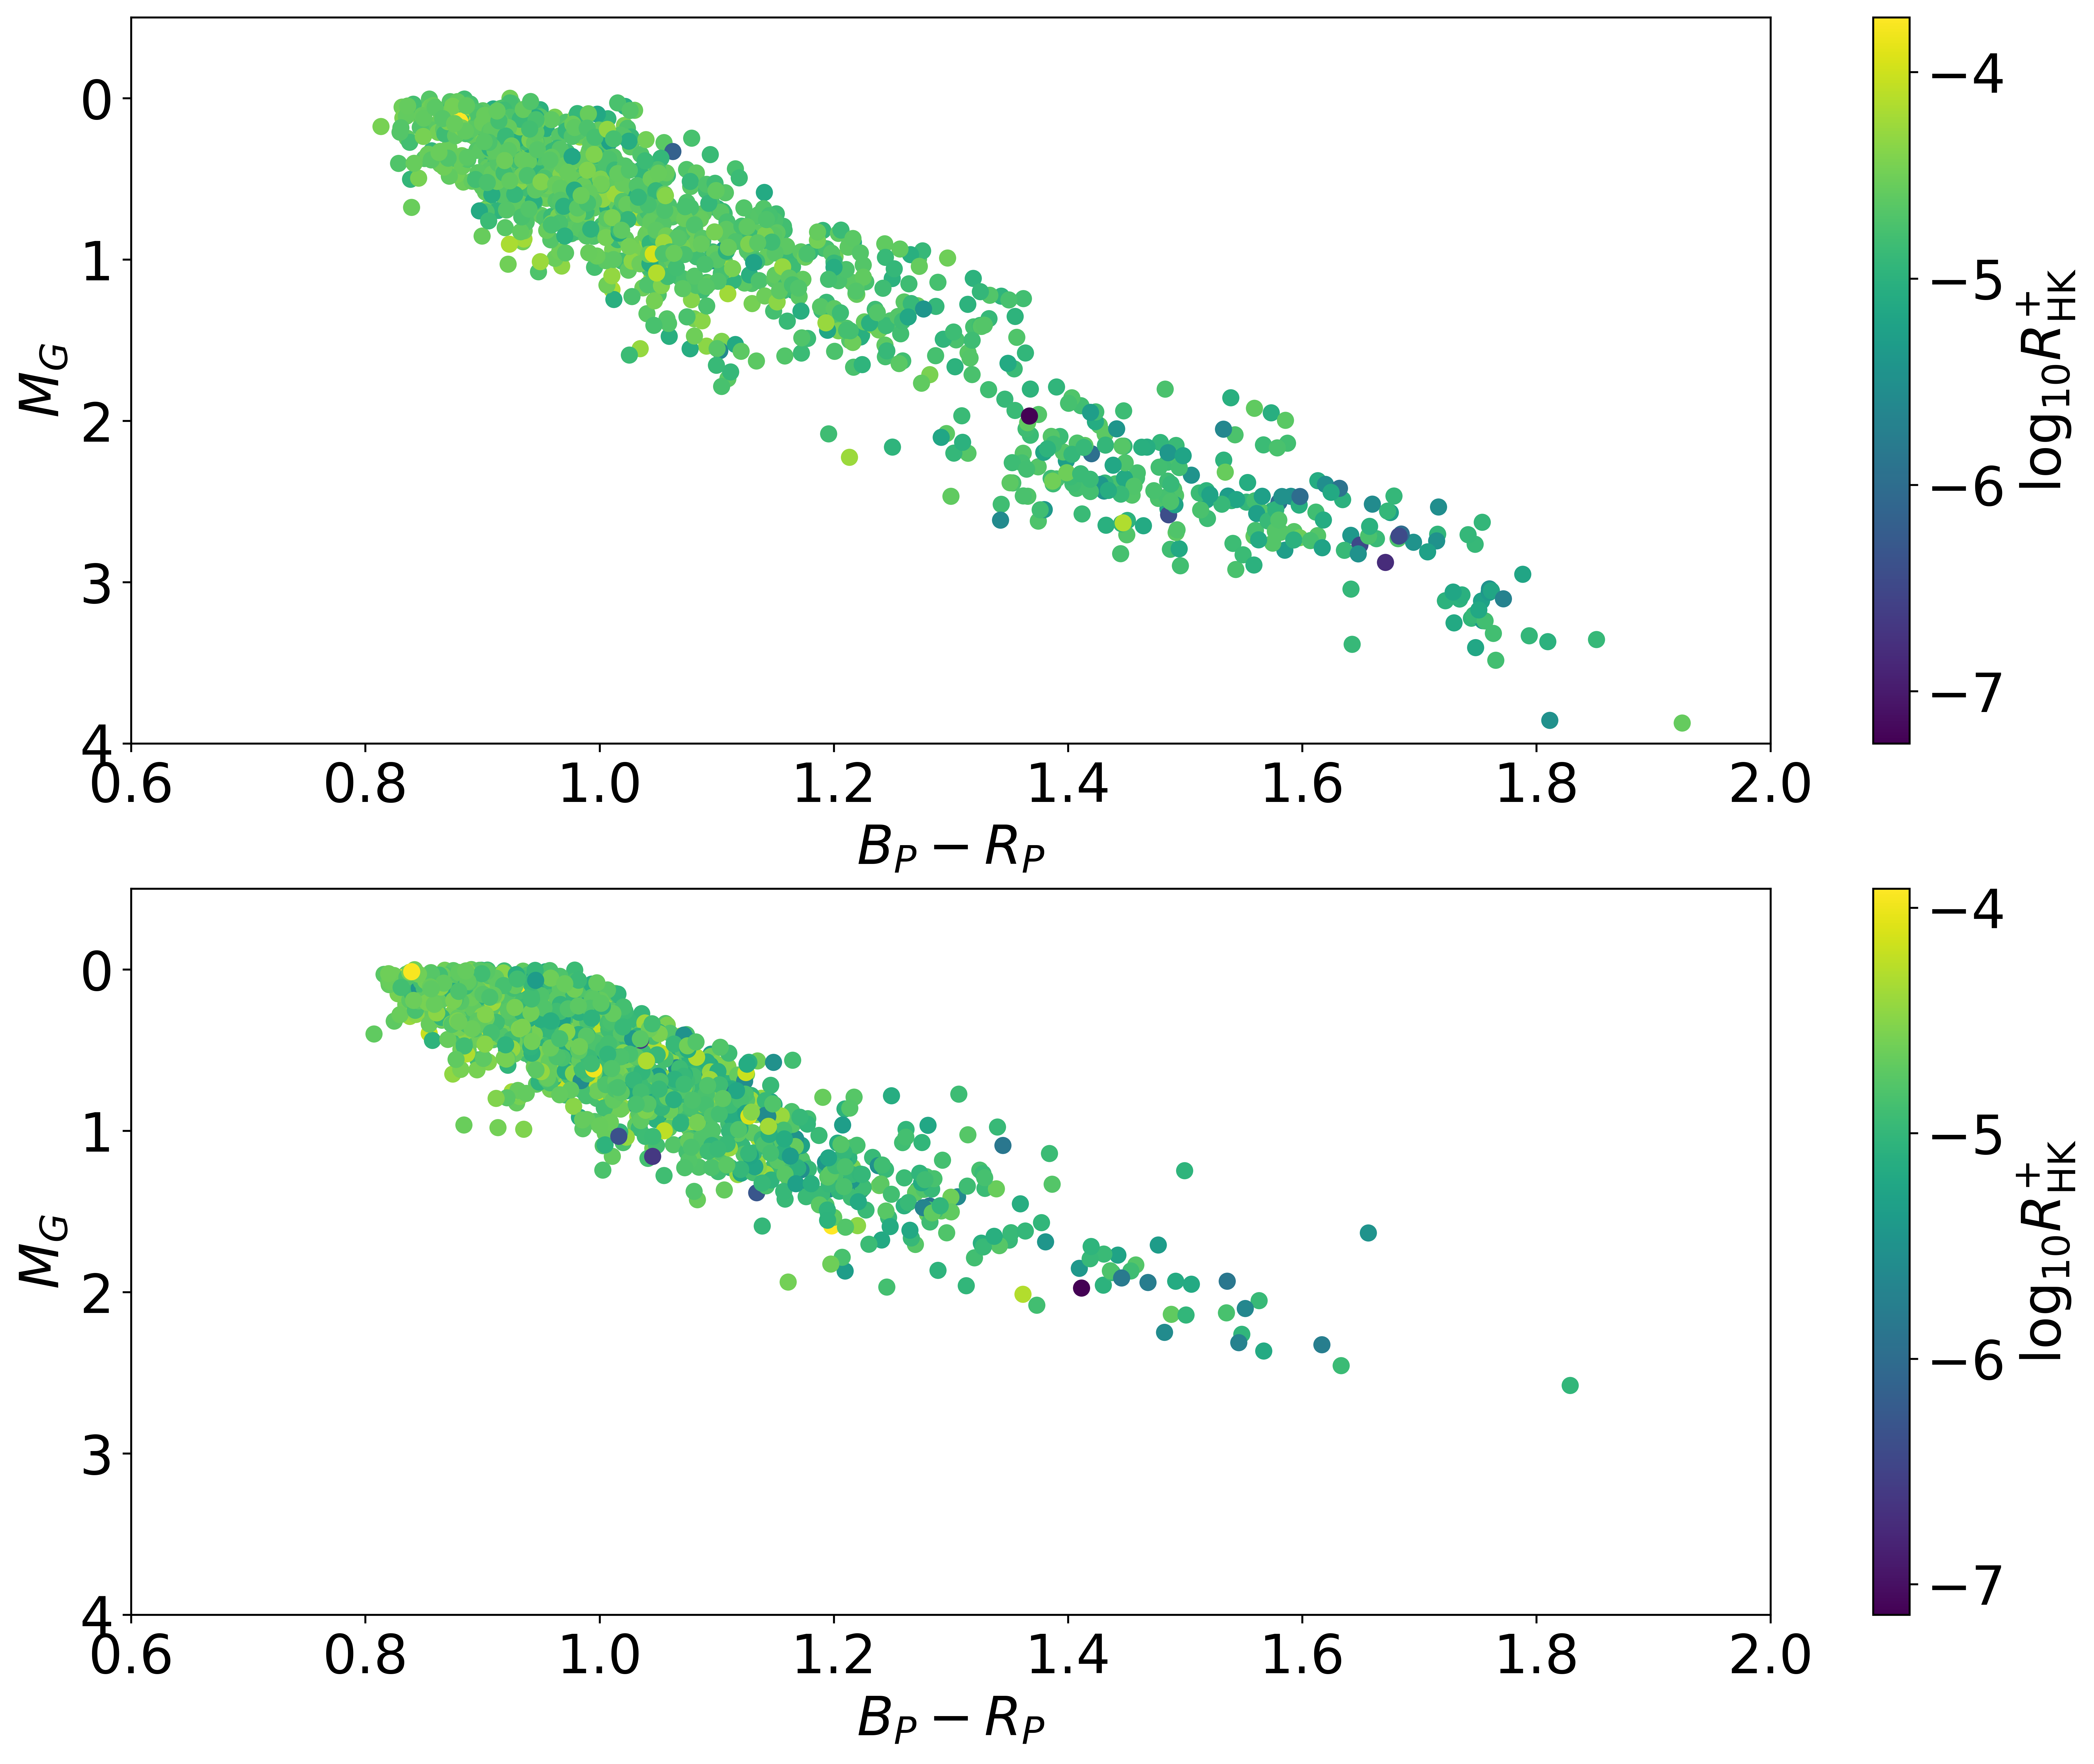
\includegraphics[width=\textwidth]{Figures/rot_gap_figures/HR_mag_and_non_rot.png}
    \caption{
    HR diagram of the closeby rotating (top) and non-rotating (bottom) main-sequence sample cross matched with the LAMOST-\kepler{} field coloured by the chromospheric magnetic activity indicator $\log \ R^{+}_{HK}$.
    Comparing this two samples we observe there are very few low mass stars for which the rotation period is not detected.}
    \label{fig:non_rotating_mag_hr}
\end{figure}


With the rotating and non-rotating LAMOST-\kepler{} samples we can investigate the detectability of rotation as a function of $\log \ R^{+}_{HK}$.
We expect more magnetically active stars (higher $\log \ R^{+}_{HK}$) to be easer to detect in rotation as \rper{} should increase in turn - however, as we have noted earlier in this work, stars can have their rotation go undetected for a multitude of reasons and the non-detection of rotation will not purely be the result of a lower magnetic activity.
Figure \ref{fig:pdf_cdf} shows the distribution of rotation detected and rotation non-detected samples with $\log \ R^{+}_{HK}$
The left panel shows the probability density while the right shows the cumulative probability density function.
Stars detected in rotation appear to have higher $\log \ R^{+}_{HK}$ than those without detection.
A Kolmogorov-Smirnov (KS) test returns a $p$-value of $4 \cdot10^{-15}$.
With this we can reject the null hypothesis that the two samples are drawn from the same underlying distribution with strong statistical significance.
The non-rotation detected tends to be less magnetically active, in terms of $\log \ R^{+}_{HK}$, than the rotationally detected sample.

\begin{figure}
\centering
    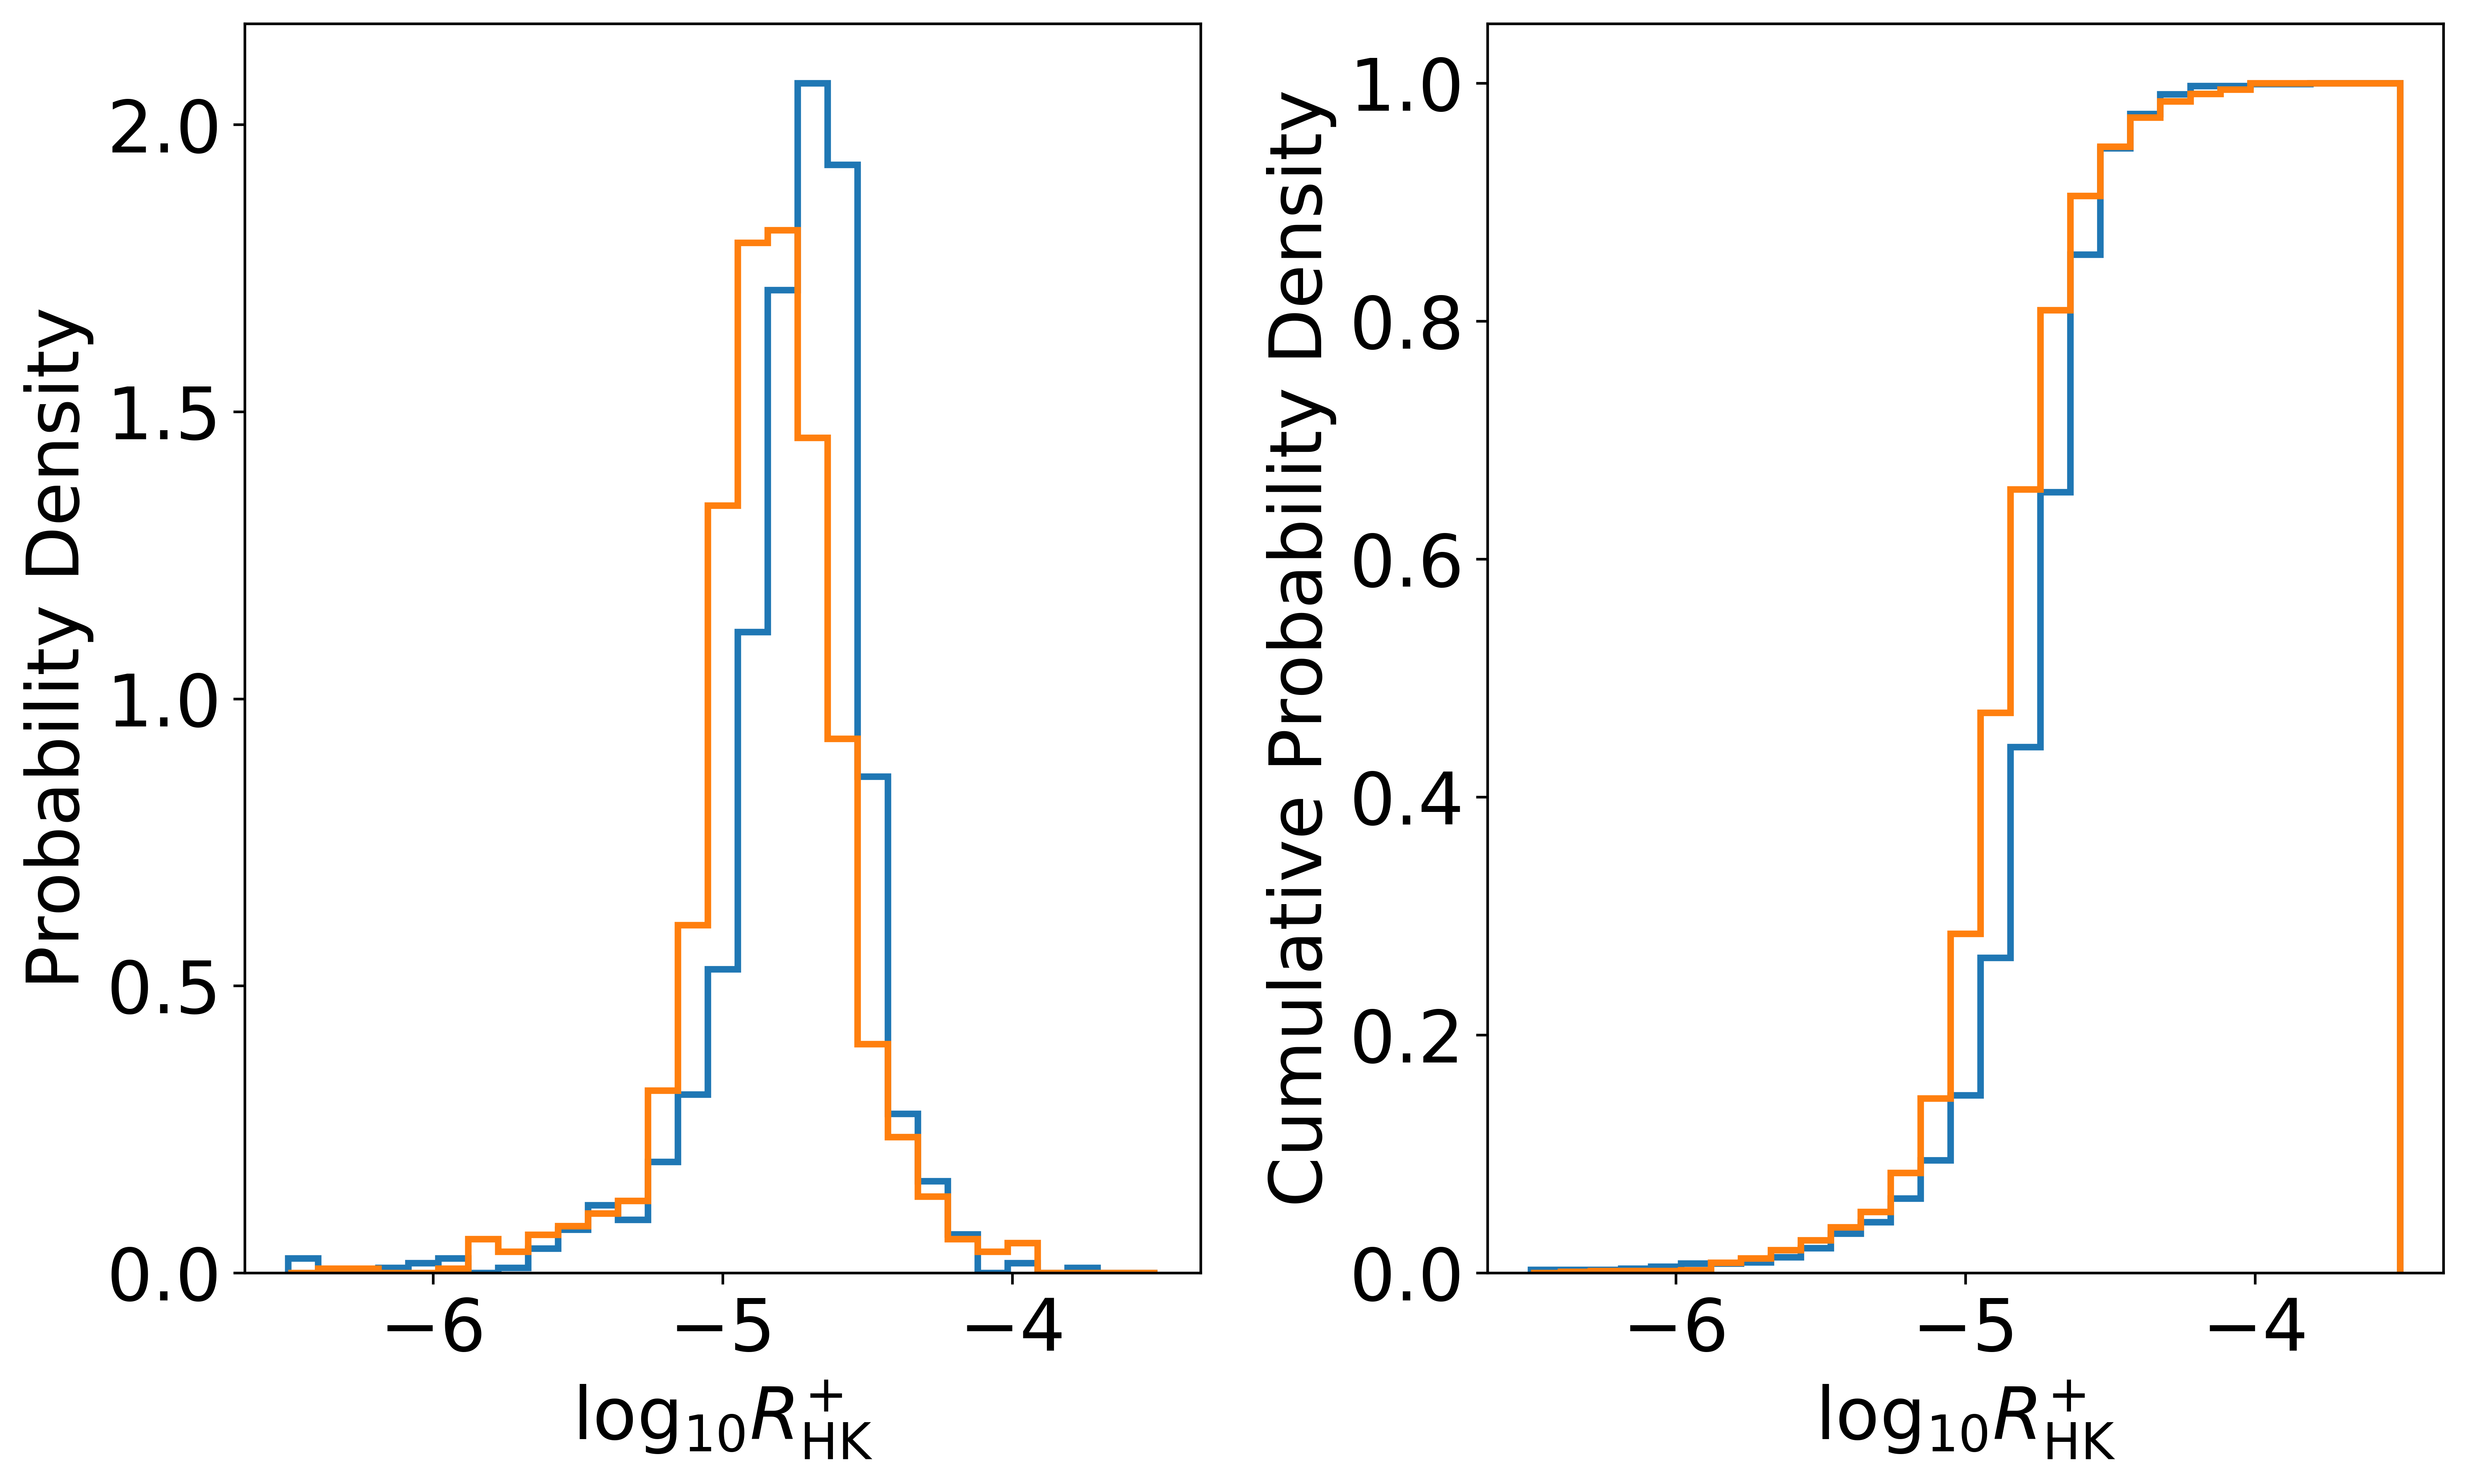
\includegraphics[width=\textwidth]{Figures/rot_gap_figures/pdf_cdf.png}
    \caption{
    	The probability density function (left) and cumulative probability density function (right) of $\log \ R^{+}_{HK}$ separated by whether rotation was or was not detected in the close-by main-sequence LAMOST-\kepler{} crossmatch. 
	We expect that less magnetically active stars to have a lower detection rate due to the decrease in prominence of stellar spots with lowering magnetic activity. This appears to be supported by the data here as the non-rotation detected sample contains a larger number of low $\log \ R^{+}_{HK}$ stars.}
    \label{fig:pdf_cdf}
\end{figure}

To investigate the detectability of rotation, let us consider the fraction of targets for which we detected periods in bins of colour and $\log \ R^{+}_{HK}$.
The detection efficiency here is measured from the ratio of the number of stars with a measured rotation rate to the total number of stars in that bin.
Other works \citep[See e.g.]{claytor_recovery_2022} consider the ratio of stars with highly precise measures of rotation period to those that do not.
We forgo any cuts to the fractional error on rotational period as we have limited our stars to nearby stars, that have very high precision recovery of stellar rotation period and make no cuts to the number of stars in each bin that we calculate the histogram for. 
While limiting the minimum number of stars would allow us to clarify large scale trends, we are searching for a subsample of stars with spuriously low magnetic activity with an already small sample size.

\begin{figure}
\centering
    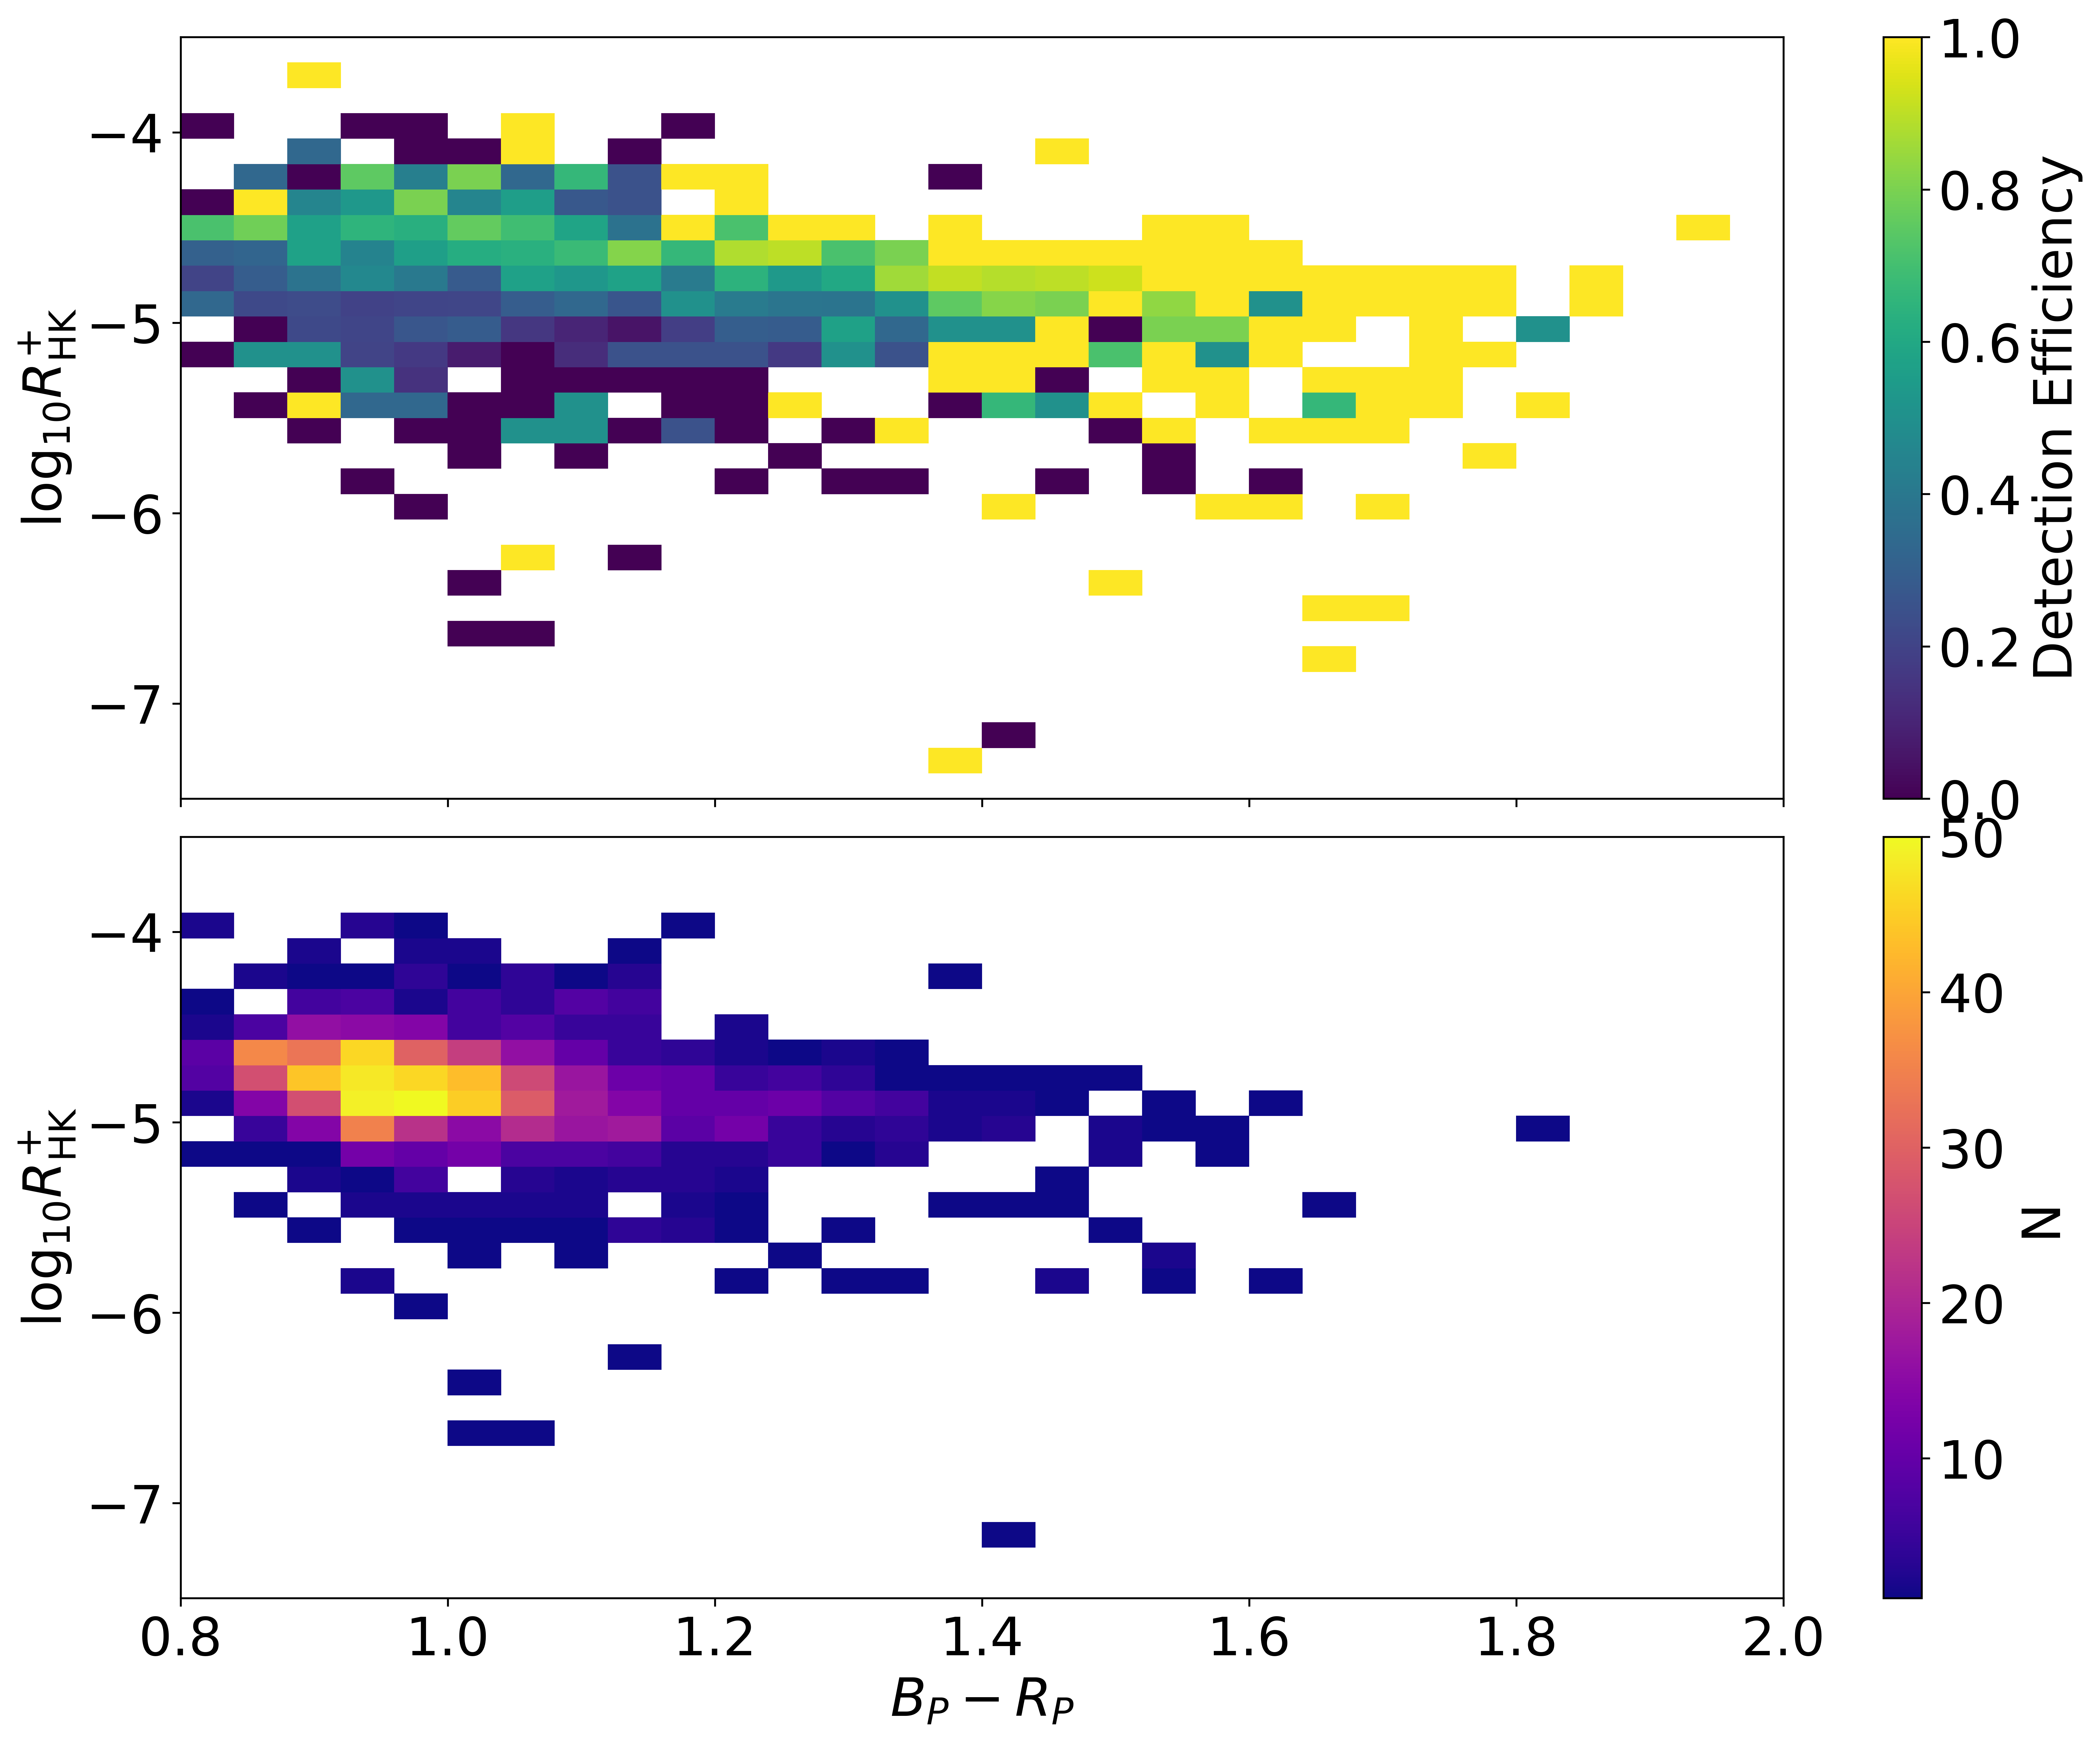
\includegraphics[width=\textwidth]{Figures/rot_gap_figures/detection_efficiency.png}
    \caption{
    	The detectability of rotation (top) and 2D histogram of stars without detected rotation periods (bottom) across \gaia{} $B_P - R_P$ colour and $\log \ R^{+}_{HK}$ . 
	Rotation is preferentially measured in stars with higher magnetic activity (larger $\log \ R^{+}_{HK}$) and tends to increase with colour. Low mass stars have a high probability of rotation being measured. Stars with low magnetic activity have a lower probability of rotational observation. Bins with detection efficiency = 0 or 1 contain single stars and are not indicative of trends in the detection efficiency.
	We do not observe an ultra low magnetic activity population with non detected rotation that would be required to explain the lack of observation of stars in the intermediate period gap.
	While there is stars with ultra low $\log \ R^{+}_{HK}$  ($<$5.5) in each $B_P-R_P$ bin they can either both rotationally detected or not rotationally detected. The ultra-low magnetic activity is not indicative of their lack of probability of their rotational observation.
}
    \label{fig:detection_efficiency_rhk}
\end{figure}

Figure \ref{fig:detection_efficiency_rhk} shows the detection fraction (top) and a 2D histogram of the non-detected rotation sub sample (bottom) against colour and $\log \ R^{+}_{HK}$. 
We confirm that rotation is preferentially measured in stars with higher magnetic activity (larger $\log \ R^{+}_{HK}$) and tends to increase with colour. 
Low mass stars have a high probability of rotation being measured - which is expected from their lower brightness resulting in larger \rper{} for the same magnetic activity and stars with low magnetic activity have a lower probability of rotational observation. 
Bins with detection efficiency = 0 or 1 contain single stars and are not indicative of trends in the detection efficiency.
We do not observe an ultra low magnetic activity population with non detected rotation that would be required to explain the lack of observation of stars in the intermediate period gap.
While there is stars with low, for a given colour bin, and ultra low $\log \ R^{+}_{HK}$  ($<$5.5) in each $B_P-R_P$ bin they can either both rotationally detected or not rotationally detected. 
The ultra-low magnetic activity is not indicative of their lack of probability of their rotational observation.
While stars older-slowly rotating stars also tend to have lower $\log \ R^{+}_{HK}$, which may camouflage a population of low $\log \ R^{+}_{HK}$ gap stars, they still tend to have observable rotation periods.
For the gap to exist the magnetic activity would need to drop to a point where observation of rotation period is impossible, which is not supported by the data here.


\section{The lack of observation of stars that could fill the intermediate period gap}
\label{sec:no_gap_stars}


In this work we have suggested that the data does not support the hypothesis that the rotational period gap is in-fact full of stars without detectable rotation periods.
If the gap is indeed full of stars without detectable rotation periods then, if we assume that the selection functions of both the time-series photometric missions (\kepler{}, \ktoo{}, \tess) nor the works that have attempted to measure the rotation periods of stars from the data collected in those missions is not biased towards not observing or measuring the rotation periods of stars in the gap then the gap stars should permeate the sample of stars without detected rotation periods.
Further, for the gap to be full of stars there must be enough stars without detected rotation periods to fill the dearth of observations.
In this Section we will determine whether this is indeed the case.

We compare the distribution of stars in the \citet{mcquillan_rotational_2014} \kepler{} rotating and undetected rotating samples.
While \citet{santos_surface_2019} has increased the sensitivity of rotational detection of stars in the \kepler{} sample this has not increased the number of observations of stars within or near the gap nor significantly increased the number of low-mass ($B_P-R_P$ $>$1.7) stars with detected rotation periods.
Our analysis will be focussed on very low mass stars where the gap is most apparent - where \citet{mcquillan_rotational_2014} remains the state-of-the-art.
We make no quality cuts to the data to ensure we are not preferentially selecting for stars that could/could not possibly fill the gap.

In their work \citet{mcquillan_rotational_2014} differentiates between rotation-detected and non-rotation-detected stars using the threshold described in the previous section. 
Low-mass stars with low-significance reported rotation periods in the undetected rotation catalogue are disproportionately distributed close to the gap, especially near $B_P-R_P$ = 1. 
Although these stars do not fill the gap, they have low $w$ and therefore seemingly support the hypothesis that the gap represents a minimum detectability of rotation period.
However, if we compare the distribution of the number of stars in the rotation detected and undetected samples with colour, as we have shown in Figure \ref{fig:n_det_nondet}, we observe that stars with detectable rotation periods outnumber stars with undetectable rotation periods at lower masses ($B_P-R_P$ $>$1.3), despite the overall 3:1 ratio of the entire detectable to undetectable catalogues.
Further in the inset of this Figure, where we compare the distributions where the gap is most apparent, we see that the proportion of stars with undetectable rotation periods to stars with detectable rotation periods decreases with decreasing mass, to a minimum of 1:10 undetectable to detectable rotation periods at the lowest masses.
However, this result in itself does not confirm whether the stars in the undetected rotational period sample fill the gap.
We instead determine how many stars would be required to fill the gap, or rather for the dearth in observations to be undetectable in the low mass range where the proportion of stars between the samples is largest and where the gap is most apparent ($B_P-R_P$ $>$1.5).


To find the number of stars required for the dearth of observations to be no longer considered a dearth we first separate the sample with detected rotation into bins of $B_P - R_P$ (colour) from 1.5-2.2 of size 0.045 (15 bins).
In each colour interval, we then split the data into log rotational period intervals of width 0.07 dex between 1.0 and 1.7 dex (10 bins) - which correspond to 10 and 50 days, respectively.
We then calculate the number of stars in each slice of log period for a given colour range and remove bins with only 1 star from our analysis.
In FIgure \ref{fig:n_col} we show the number of stars in each slice (scatter points) against $\log_{10}$ of the rotation period for each colour range indicated in brackets to which we have fit a cubic spline (dashed)
From the cubic spline, we can use the first and second derivatives of the spline to accurately determine the position of the local minima in density, which is indicated by the solid vertical black line.
The calculation of the position of the minima is again an automated process as carried out in the previous Sections.
To calculate the number of stars required for the dearth/minima to be no longer apparent we compare the number of stars in the closest scatter point to the minima to the average of the two scatter points surrounding it.
While this approach is admittedly naive, it assumes all of the stars will be in the bin closest to the minima rather than being distributed throughout the dearth region, it places a lower bound on the stars required to be observed for the gap to be filled and accounts for the decrease in the number of stars observed at lower masses.

In Figure \ref{fig:stars_not_fill} we compare the number of stars required to fill the gap to the number of stars without detected rotation periods in each colour range.
We find that the number of stars required to fill the gap is approximately constant at N $\sim$ 20.
This suggests that the number of stars required gap is independent of the total number of stars observed in that mass range.
If the gap is full of stars without detectable rotation periods we expect the proportion of stars required to fill the gap to increase proportionate to the total number of stars (detected and non-detected rotation) but this is not the case.
The number of stars required to fill the gap is much smaller than the number of stars without detected rotation periods for $B_P-R_P<1.8$.
As colour increases and the number of observed stars decreases the number of stars required to fill the gap becomes the majority of stars without detected rotation periods.
This suggests that for the gap to be full of stars with undetected rotational period stars, all of the stars in the undetected rotational period sample would need to be in this small rotational period range and only a very small number of stars with undetected rotation are the result of noise or inclination effects.

Two conclusions could be drawn from this result.
The gap is full of stars with undetectable rotation but most to all of the stars with undetectable rotation must lay within the gap for this to be true.
The other is that the stars in the gap do not exist - they pass through the gap so quickly that stars with rotation periods that would place them in the gap evolve so quickly that their rotation periods are rarely observed.
The data appears to favour the latter, supporting the hypothesis that the gap is caused by the sudden onset of strong magnetic braking.

\begin{figure}
\centering
    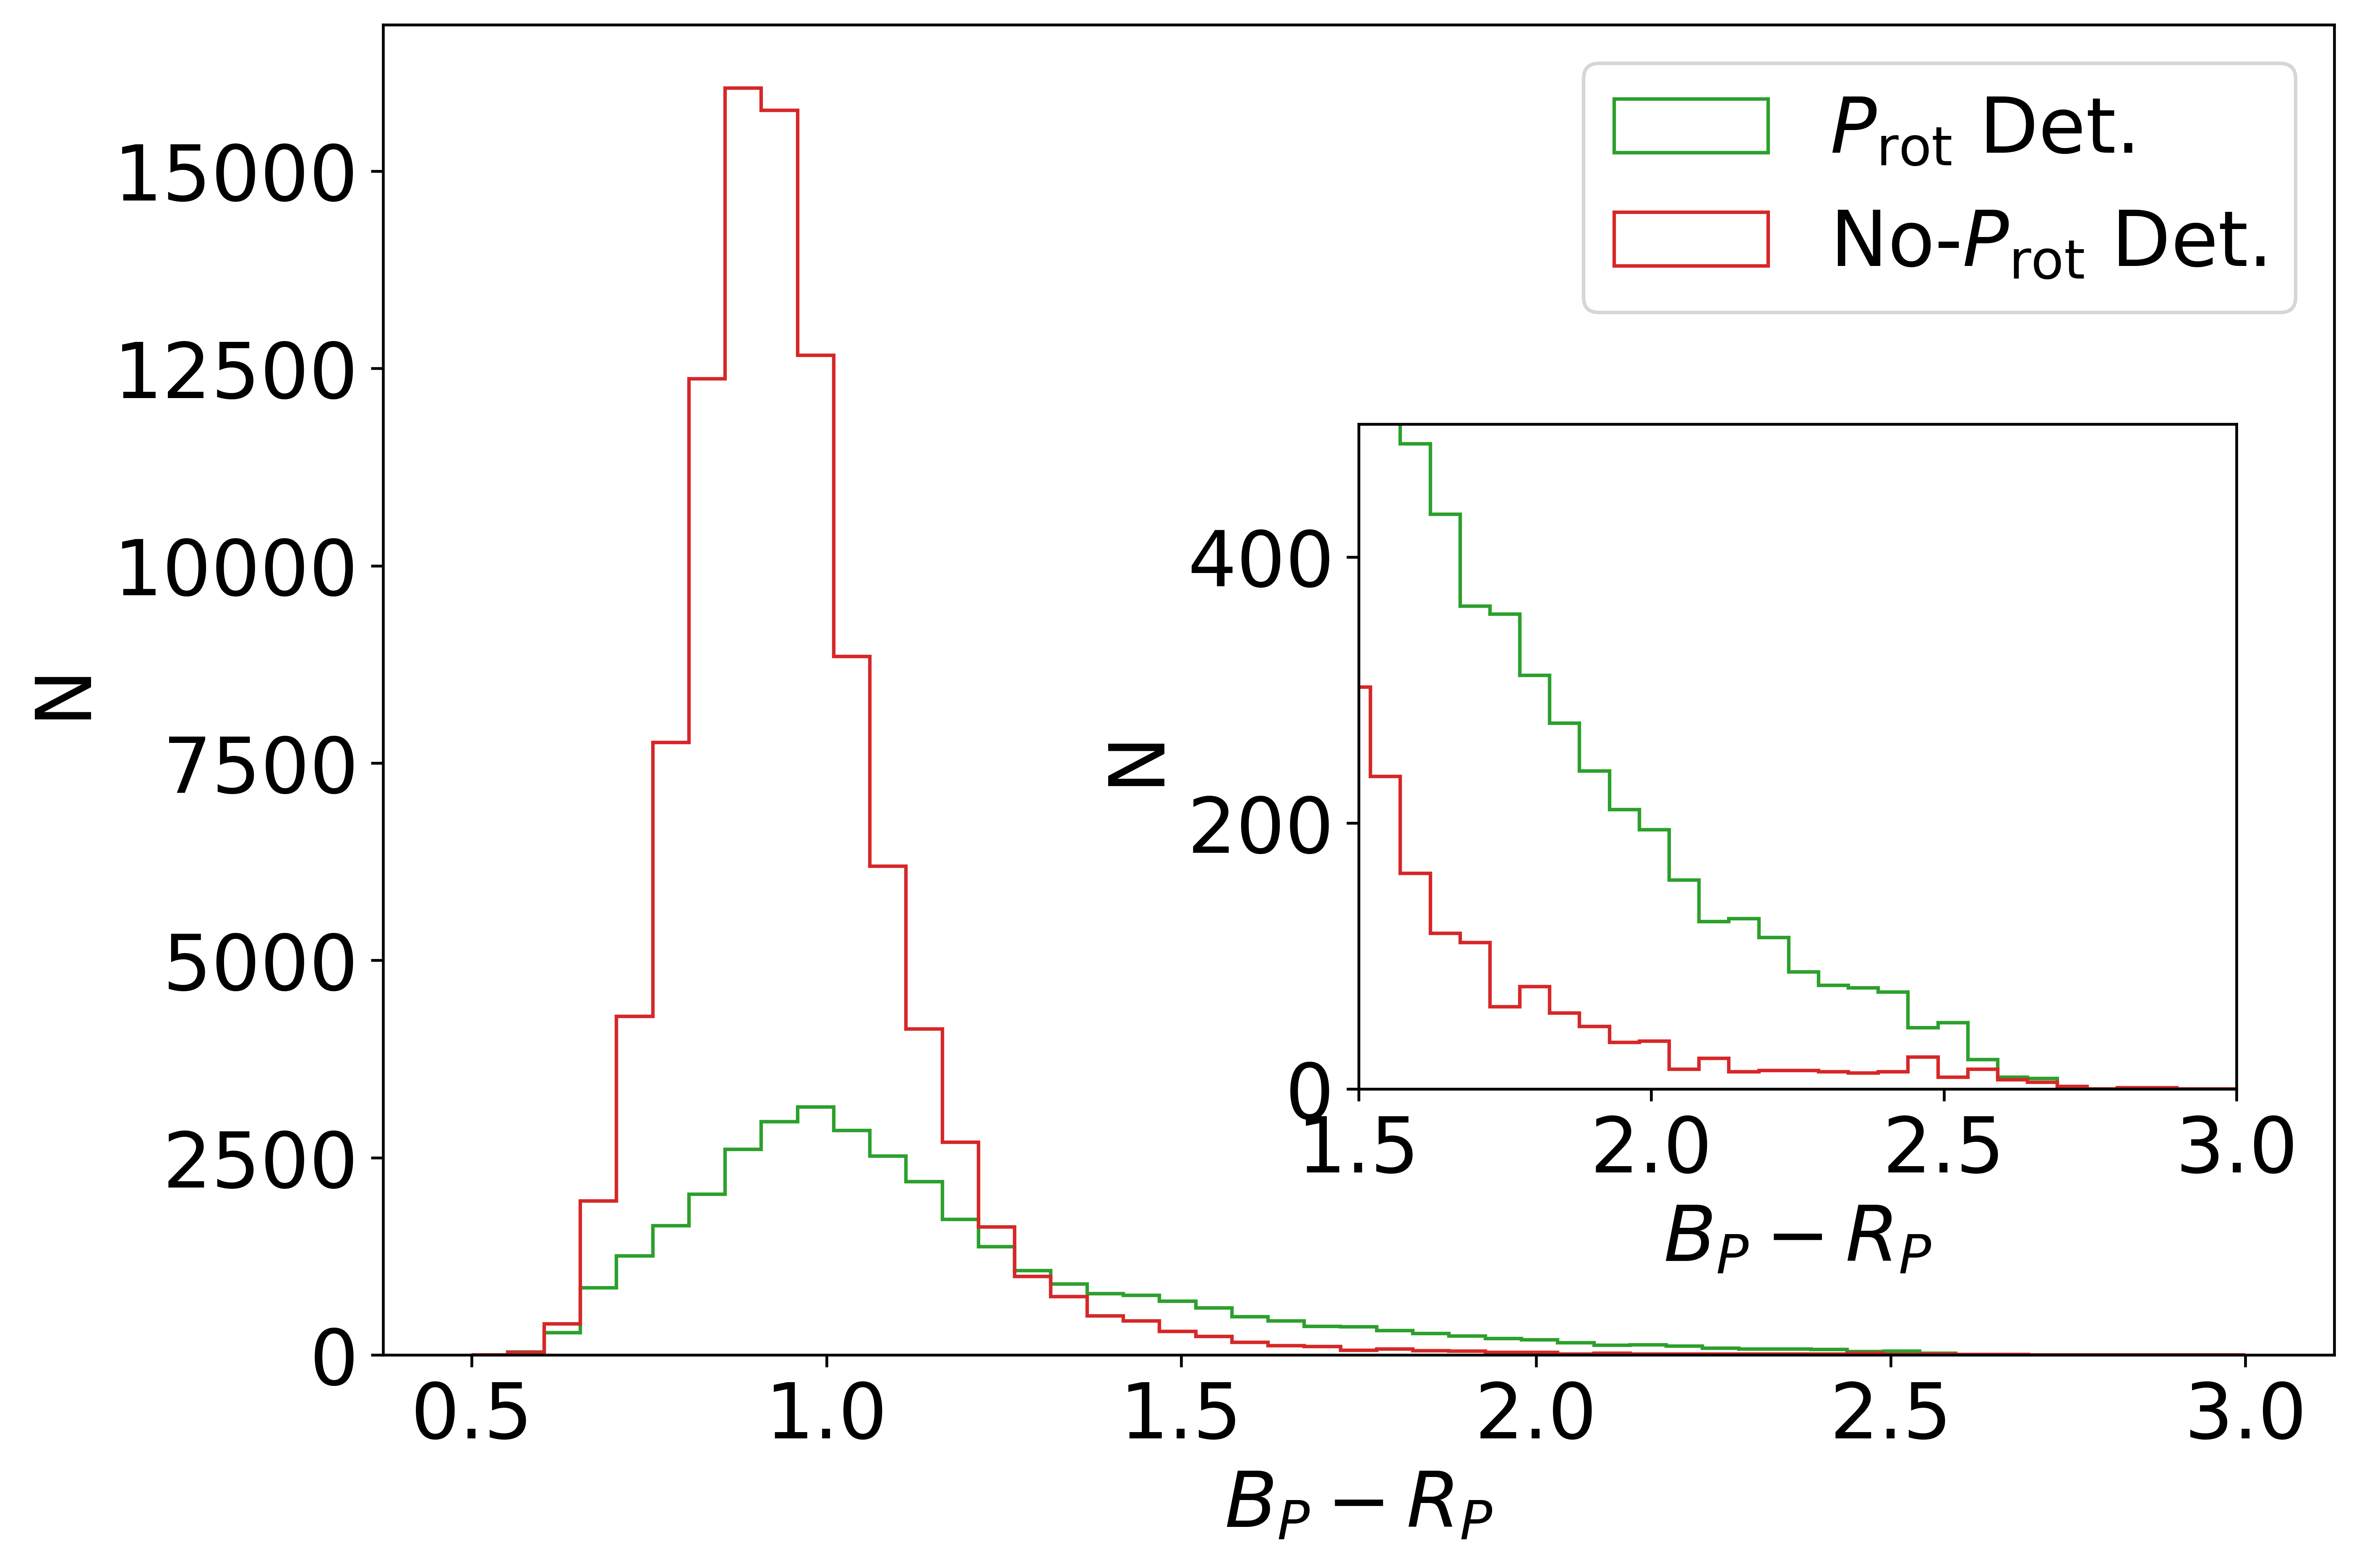
\includegraphics[width=0.5\textwidth]{Figures/rot_gap_figures/hist_obs.png}
    \caption{A histogram of the distribution of $B_P-R_P$ colour of stars with (green) and without (red) detected rotation periods. \textbf{Inset:} A zoom-in of the distribution for $B_P-R_P>1.5$ where the rotational period gap is most apparent. The distribution in colour of stars with and without detected rotation periods vary. The undetected rotation sample is strongly biased towards stars with $B_P-R_P$ close to 1, comparative to the lower-mass stars where the number of stars drops quickly. Despite the $\sim$3:1 ratio of the number of stars with undetected rotation periods to those with detected rotation periods, the number of stars without detected rotation periods drops below those with detected rotation at $B_P-R_P>1.3$.
    	}
    \label{fig:n_det_nondet}
\end{figure}



\begin{figure}
\centering
    \includegraphics[width=\textwidth]{Figures/rot_gap_figures/n_col.png}
    \caption{
    	Number of stars in each bin against $\log_10$ of the rotation period in bins of colour \gaia{} $B_P-R_P$ (indicated in brackets). Here we have fitted a cubic spline to the number of stars in each bin and calculated minima using the first and second derivatives of the fitted cubic spline. The minima in number of stars are shown by solid vertical blue lines. These minima are the rotational period gap.
}
    \label{fig:n_col}
\end{figure}


\begin{figure}
\centering
    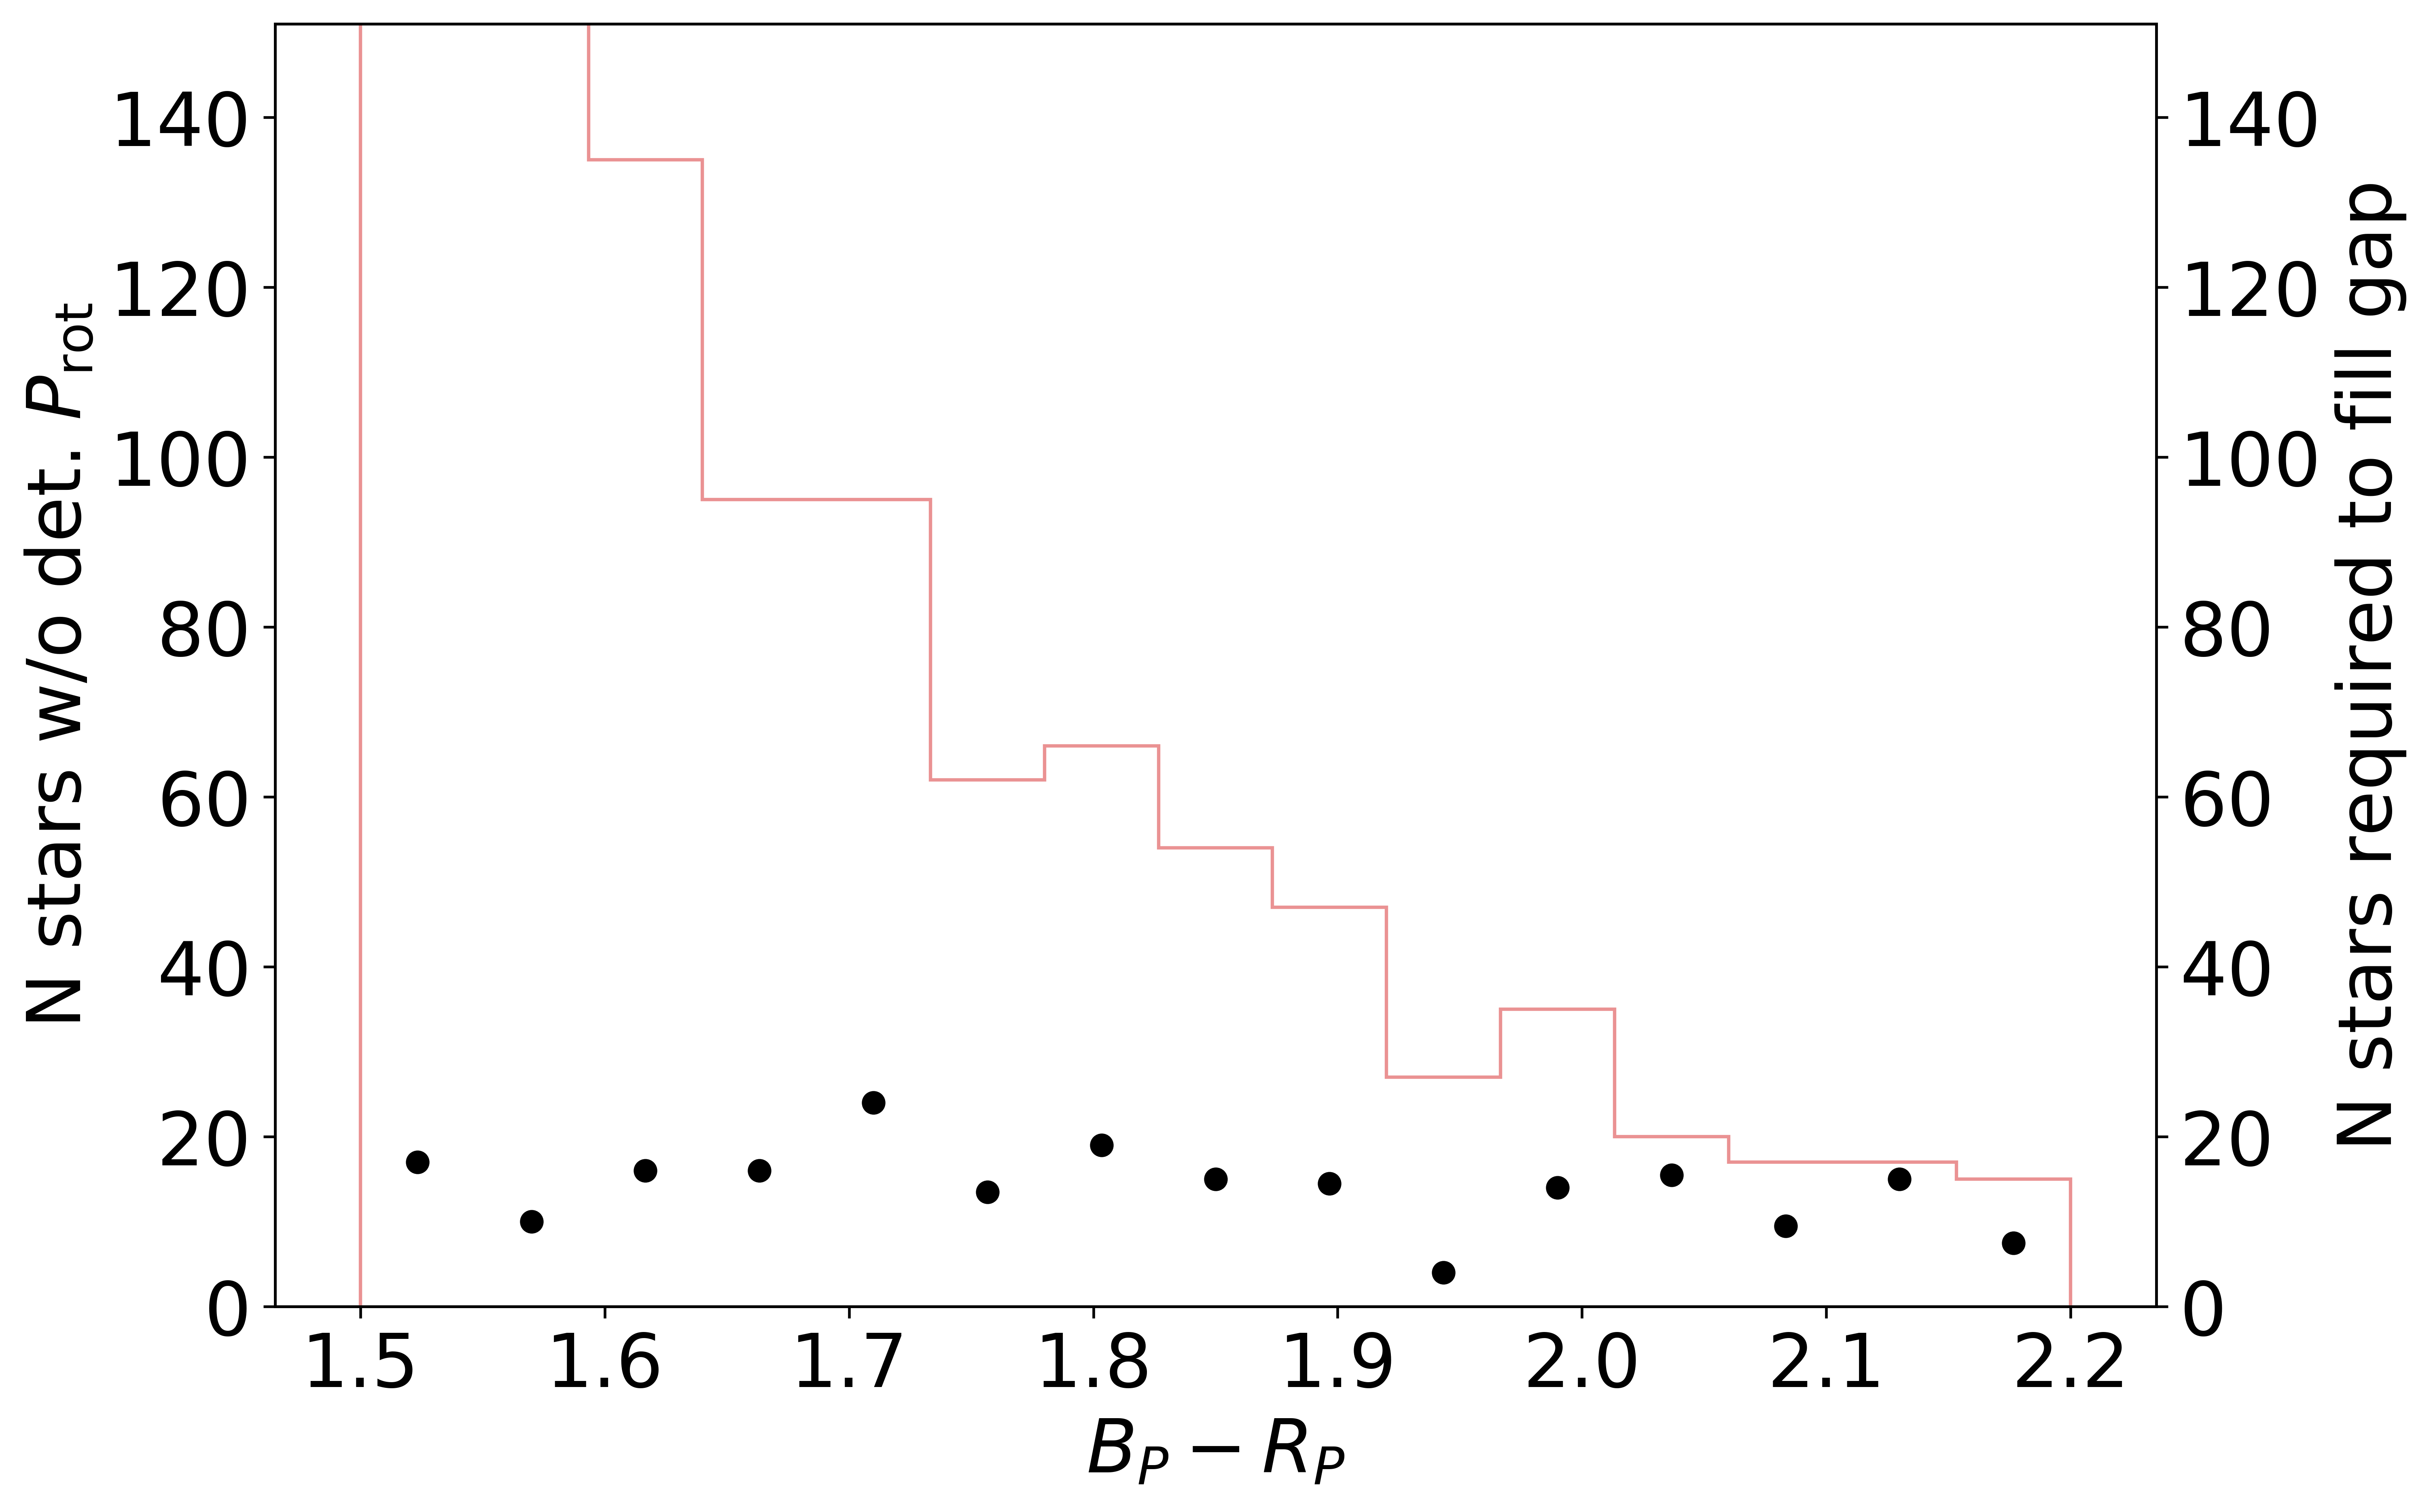
\includegraphics[width=0.5\textwidth]{Figures/rot_gap_figures/stars_donot_fullgap.png}
    \caption{
    	The number of stars required to fill the gap (black scatter points) against the number of stars with undetected rotation periods against $B_P-R_P$. The number of stars required to fill the intermediate period gap is roughly constant at N $\sim$ 20. While the number of stars without detected rotation greatly outnumbers the number required to fill the gap below $B_P-R_P \sim 1.8$, the two are almost equal for lower mass stars.
}
    \label{fig:stars_not_fill}
\end{figure}


%\section{A spectroscopic rotation of stars near the rotational period gap}


\section{Discussion and Summary}
\label{sec:disc_sum}

In this Chapter, we have investigated the distributions of the magnetic activity of stars in regard to their rotational period - specifically near the rotational period gap.
We have reconfirmed that, in regards to the surface rotation period, the gap aligns itself with a minima in photometric variability range (\rper{}).
The coincidence of the gap and the minima has been invoked to suggest that the gap is the result of a very-low probability to observe stars within the gap and that the gap is in-fact full of stars with undetectable rotation periods.
The average \rper{} of stars around the gap does not fall below the detectability threshold of rotation - stars with much lower \rper{} have detectable rotation periods can be detected.

One explanation could be that \rper{} could drop suddenly and dramatically, below the rotation detectability threshold, for stars precisely within the gap.
Whether this be from a drop to the magnetic activity of stars within the gap to little to no expression of stellar spots or, as \citet{reinhold_spot_2018} suggests, the result of the cancellation brightness variations of spots by faculae is currently unknown.
We found in this work that the drop in \rper{}, and thus the gap, is also coincident with a drop in $\log R^{+}_{\rm{HK}}$ suggesting that the decrease in photometric variability in stars close to the gap is the result of a decrease in magnetic activity, rather than a transition in the spots dominance to faculae dominance.
However, we also found that there is not a subsample of stars without rotational period detection but with ultra-low $\log R^{+}_{\rm{HK}}$.
While the stars without rotational period detection tend to have lower magnetic activity, there is not an obvious subsample of stars with $\log R^{+}_{\rm{HK}}$ below the rotation period detection threshold.
This suggests that there are no stars within the gap with ultra-low magnetic activity that make rotational period observation impossible.

\citet{reinhold_spot_2018} proposed an explanation for the gap in which the amplitude decrease of \rper{} can be explained towards the gap if we assume that stars are spot-dominated below the gap, undergo a period of spot-faculae cancellation before returning to spot-dominance above the gap.
In this work, they show they show that faculae-spot cancellation can lead to the non-detection of rotation but \textit{do not} find evidence of spot-faculae cancellation close the rotation period gap.
Further, they do find evidence of a transition from spot to faculae dominance for much older stars at the Vaughn-Preston gap ($R_o \sim 2$) but do not find a variation in \rper{}, nor a dearth of rotators, around the Vaughn-Preston gap.
This suggests that a transition from faculae to spot dominance does not in fact affect the photometric variability of stars with observed rotation periods.
If the gap is indeed caused by the transition from spot to faculae dominance then the decrease in \rper{} would not be met by a decrease in other magnetic activity indicators.
They propose that the transition from spot to faculae dominance is representative of a transition from large and long-lived spots to small, short-lived spots with longer-living faculae which introduce noise and cancel out the brightness variations to the spectra, resulting in low detectability of rotation.
Our work does not support this hypothesis.
The decrease in \rper{} are coincident with a drop in the magnetic activity of stars near the gap, suggesting that the decrease in \rper{} instead caused by a decrease to the expression of stellar surface features. 

Another possible mechanism we can investigate using this data arises if we consider that stars within the gap may have magnetic activity so great that noise dominates their light curves making observation of their rotation impossible.
Rotation tends to be less readily detectable at times of high activity when the light curve is noisy from the stochastic production of a larger number of surface features.
Consider a scenario whereby the average magnetic activity of stars increases in the region of evolution around the magnetic activity gap - indeed the magnetic activity of stars tends to decrease with rotation rate but we will ignore this for now.
Let us assume instead that the spot-faculae cancellation does not occur and that brightness variations on a magnetic activity timescale are spot dominated below the Vaughn-Preston Gap \footnote{A distinct gap from the intermediate period gap wherein the transition from spot dominance to faculae dominance occurs in their work} .
Conceivably, as the average magnetic activity increases for stars near the gap the regions where noise is minimal enough for rotation to be detected become smaller and more concentrated to times when the magnetic activity of stars is very small - which must constitute a minority of stars for a given $B_P-R_P$ and rotational period.
This would coincide with a decrease in \rper{} of stars as average magnetic activity increases.
The gap would then represent a region of evolution where the average magnetic activity of stars would then be large enough that the noise permeates the entire magnetic activity cycle and no observations of rotation could be made.
Observations of rotation period should therefore be more likely occur when a star is minimally active and thus have smallest observed magnetic activity- which would also correspond to a minima in observed $\log R^{+}_{\rm{HK}}$.
This would suggest that there is a population of magnetically active stars with $\log R^{+}_{\rm{HK}}$ greater than the average magnetic activity of stars near the gap that have otherwise undetectable rotation periods.
In Figure \ref{fig:detec_rhk_min_shown} we show that there is not a subsample low rotation detectability stars with $\log R^{+}_{\rm{HK}}$ greater than the average of stars near the rotational period gap - suggesting that this selection mechanism is not at play.

Another feature that is consistently observable in the variance of \rper{} with rotation period across the rotation period gap is a maxima in \rper{} for stars with rotation periods that place them above the gap.
These maxima are unexplained by a model where the gap is the result of a decrease in the observability of rotation in stars near and within the gap.
If indeed the gap represents a transition from spot to faculae dominance, then the mechanism for detectability decreasing is a suppression \rper{} by faculae on spots.
Largely speaking, as rotation period increases, magnetic activity decreases and photometric variability also decreases.
For stars to have detectable rotation periods above the gap, the suppression of photometric variability by faculae on spots should restore \rper{} to levels observed below the gap.
This feature is also coincident with an increase in $\log R^{+}_{\rm{HK}}$ for those stars.
The photometric variability increase is expected under an increase to  $\log R^{+}_{\rm{HK}}$, suggesting again that the mechanism underlying to the two features is connected.

The proposition that the rotational period gap represents a minima of detectability of stars is not favoured by the data.
Increases to detector efficiency have also not increased the observation of stars near, nor in, the intermediate period gap as each model proposed to explain the minima of detectability of rotation period predicts.
The coincidence of the minima in \rper{} with minima in $\log R^{+}_{\rm{HK}}$ along with the lack of a population of low or high $\log R^{+}_{\rm{HK}}$ stars with low detectability suggests that minima in \rper{} cannot be explained by a spot-faculae transition nor a selection effect for stars with low or high magnetic activity near the rotational period gap.
Furthermore, the number of stars required to fill the gap is larger than the number of stars without detectable rotation periods.
Recent works have also tentatively shown that the kinematic ages of stars above and below the rotation period gap have comparable kinematic ages \citep{lu_bridging_2022}.

The only alternative mechanism that has been proposed and is not disfavoured by the data arises from the onset of sudden magnetic braking whereby stars jump the gap.
However, this explanation is complicated by the fact that we do not know the mechanism underlying the sudden magnetic braking.
As stars evolve toward the gap, their core and envelope have undergo recoupling, slowing their spin-down.
\citet{cao_core_2023} suggest that the process of core-envelope recoupling with significant angular momentum flux (See Section 4. of their work) between the core and the surface enhances the magnetic dynamo of stars, inducing larger photometric variability from greater spot coverage.
The decrease in photometric variability towards the gap can be explained under this framework if the enhancement of the magnetic dynamo is dependent on the scale of the radial shear between the core and the dynamo which decreases towards the magnetic activity gap.

Two mechanisms could be invoked to explain the sudden enhanced spin-down: core-envelope decoupling or enhanced magnetic spin-down.
Conceivably the core and the surface of the star can again decouple at the rotational period gap; the surface spins down at a much faster rate than below the gap resulting in the apparent dearth of observations.
It is, however, not clear the effect that this decoupling would have above the gap.
If the core and envelope are strongly decoupled above the gap then angular momentum transport between the core and surface is likely to reoccur, supported by the relatively flat radial rotation profile observed for the Sun and other solar-age stars \citep{hall}.
\rper{} of stars just above the gap is similar to stars below the gap, suggesting that they do not have enhanced dynamos consistent with the strong radial shears.
Further \rper{} increases with rotation period above the gap, suggesting instead that the enhancement of the dynamo by core-envelope should grow as the star evolves.
For this to be the case the core-surface radial shear must grow and the core and surface must remain decoupled until recoupling enhances the magnetic dynamo.
However, the gap is only apparent for a small rotational period range and the density of stars with observed rotation periods above and below the gap are consistent - suggesting that the decoupling is not slowly counteracted by core-envelope recoupling resulting in the enhanced \rper{} away from the gap.

Enhanced magnetic angular momentum loss is another possible explanation for the gap.
The magnetic braking of a star is dependent on the rotation rate, mass loss rate and the strength of the magnetic field.
Stars near and just above the gap are rotating slower and have smaller magnetic activity indicators than stars below the gap.
If this is indeed the



In this Chapter we have explored the relation between the rotational period gap and changes to the magnetic activity of stars.
We found that the magnetic activity of stars, measured here through both \rper{} and  $\log R^{+}_{\rm{HK}}$, decrease towards the gap.
Suggesting that the formalism underlying the two

under the framework


%
%
%If this were the case then core envelope coupling would begin again
%
%
%, resulting in the decrease of the strength of the magnetic dynamo and thus a decrease in photometric variaibility.
%Let's assume then at the lower edge of the gap the core and the envelope can again decouple.
%The surface convective region has a much smaller moment of inertia than the whole star.
%For the same amount of angular momentum loss from wind braking - and without angular momentum transport from the core to the surface - the surface of the star can spin down rapidly comparative to the spin down observed proceeding the gap.
%Following the gap then the core and envelope can undergo recoupling: enhancing the magnetic dynamo and resulting in the increases to \rper{} we observe for stars above the gap
%
%
%
%
%The variance to magnetic activity we have discussed in this Chapter may in fact be explained under this framework.
%
%As stars evolve toward the gap, their core and envelope have recoupled, resulting in the decrease of the strength of the magnetic dynamo and thus a decrease in photometric variaibility.
%Let's assume then at the lower edge of the gap the core and the envelope can again decouple.
%The surface convective region has a much smaller moment of inertia than the whole star.
%For the same amount of angular momentum loss from wind braking - and without angular momentum transport from the core to the surface - the surface of the star can spin down rapidly comparative to the spin down observed proceeding the gap.
%Following the gap then the core and envelope can undergo recoupling: enhancing the magnetic dynamo and resulting in the increases to \rper{} we observe for stars above the gap
%
%then assume the core and surface decouple then the core and envelope were to decouple, where the surface spins down relative to the core
%
%
%
%
%
%
% this proposed mecha
%
%
%
%
%
%
%
% variability of stars on a rotational timescale would decrease across all stars
%
%
%
%
% this is not in fact a selection effect.
%
%
%
%In such a scenario the scatter in
%
%In Sections \ref{sec:minima_RHK} and \ref{sec:low_activity_gap} we explored the cross-match of the undetected rotation period and LAMOST $\log R^{+}_{\rm{HK}}$ samples and found that the minima in \rper{} also align with minima in $\log R^{+}_{\rm{HK}}$ and showed that there is no subsample of ultra-low magnetic activity stars that would be required to explain the drop in detectability of rotational periods.
%Let's reconsider the analysis under this new framework.
%The alignment of minima of \rper{} and $\log R^{+}_{\rm{HK}}$ in regards to the rotational period would then be explained by the bias introduced by the necessity of observation of the rotational period. 
%The detection of rotation period near the gap requires we observe stars with low magnetic activity and thus low \rper{} and $\log R^{+}_{\rm{HK}}$.
%Under this framework: stars with observed rotation periods near the gap are a subset of stars inherently selected for low-magnetic activity and there must be a subset of stars with high magnetic activity but low rotational detectability.
%However, if we plot the detectability of stars against colour and $\log R^{+}_{\rm{HK}}$ there is not a subsample of stars with larger magnetic activity than the magnetic activity of stars within the gap (indicated by orange scatter points).
%Indeed the detectability of rotation in stars with magnetic activity above the magnetic activity of stars within the gap is close to one.
%This suggests that
%
%
%
%
%
%
%The authors do not appear to suggest a reason for spot-dominated stars appearing above the gap nor a mechanism for the increase in rotational photometric variation amplitude above the gap.
%Further, the variability levels on both sides of the gap are not close to the detection limit: periods are detected for stars with similar properties at much lower \rper{} values.
%
%This does not appear to be the case in their work however.
%This does not however explain the increase in 
%
%The coincidence of the drop in \rper{} and $\log R_{\rm{HK}}$ suggests that the two are related.
%\citet{reinhold_spot_2018} suggests that the drop in \rper{} is the result of the cancellation of brightness changes from stellar spots by faculae (and vice versa) which they suggest is the result of a change of the topology of the magnetic field leading to expression of smaller stellar spots.
%A change to the magnetic field topology
%
%
%
%Another explanation could come in the form of us only measuring the rotational periods of low-activity stars near the gap.
%
%
%
%
%Under this explanation, there must be an upper limit on the detectability of rotation relative to the magnetic activity of stars in the noise that increased activity imparts on the lightcurve on a rotational timescale.
%The average magnetic activity of stars must also increase towards the gap such that at the minima of the activity cycle, the noise imparted on the lightcurve is greater than the 
%
%
%
%
%
%Under this explanation, there must be a subsample of high magnetic activity stars from which we do not detect rotation and all gap stars must have average magnetic activities that place them above the
%
%then, the stars within the rotational period gap would be
%
%
% the minima in \rper{} with rotational period align themselves with the position of the rotational period gap and confirmed that this is not the result of a bias in the colour of stars in bins of constant rotation rate brought about through the shape of a dearth of observations,
%
%
% (2) report the possible detection of minima in $\log \ R^{+}_{HK}$  with rotational period that also align themselves with the rotational period gap and (3) explore evidence for the lack of observation of ultra-low magnetic activity stars with no detected rotation period that would be required to explain the low probability of observing stars within the rotational period gap.
%
%If minima in $\log \ R^{+}_{HK}$ are not spurious then this suggests that the drop in \rper{} and $\log \ R^{+}_{HK}$ arise from the same mechanism.
%Are indirect measures of the magnetic activity of stars but they arise from indirect sources.
% \rper{} is related to magnetic activity of stars because stars with larger magnetic field strength tend to express larger and and a larger number of stellar spots.
% Larger spot coverage results in larger variations to the stellar brightness .
% $\log \ R^{+}_{HK}$ is a measure of the magnetic field strength from the response of the absorption of light by Calcium H and K lines to that magnetic field.
% \rper{} is arguably more indirect a measure of magnetic field strength than  $\log \ R^{+}_{HK}$, but is more precisely and accurately measured for a much larger number of stars with detected rotation periods.
% 
% 
%We found in this work that the two appear to be directly tied.
%Increases and decreases in one with rotation period correspond to the same response in the other.
%The coincidence of the minima with the rotational period gap suggests that the cause of the drop in \rper{} is directly tied to a reduction in magnetic field strength near the gap rather the a variation to the expression of stellar spots or faculae.
%
%From the coincidence of the minima in \rper{} and $\log \ R^{+}_{HK}$ we investigated the hypothesis that stars within the gap suddenly and dramatically drop in magnetic activity to the scale that their rotation periods are undetectable.
%To do this we looked at the rotation detection efficiency of stars relative to colour and $\log \ R^{+}_{HK}$.
%We did not find evidence of an ultra-low magnetic activity sample of stars in the non-rotational period detected \kepler{}-LAMOST crossmatch that would be required for this hypothesis to be true.
%While $\log \ R^{+}_{HK}$  tends to be lower for stars with out detected rotation periods rotation period spuriously low $\log \ R^{+}_{HK}$ stars can still have their rotation periods detected - there is not a subsample of stars below the detector sensitivity.
%
%We cannot discount the possibility is stars within the rotational period gap express $\log \ R^{+}_{HK}$ so small that it falls below the detection threshold of the LAMOST measurements.
%A survey with more sensitive detection of magnetic activity through, say, Zeeman splittings of stellar absorption lines from high resolution spectroscopy would be required to discount this possibility.
%However, this process could easily become cyclical.
%Say we don't observe the required ultra low-magnetic activity through more precise measurements of the magnetic activity - then again the same explanation could be invoked.
%
%
%
%
%
%An alternative explanation for the coincidence of the minima comes from the
%
%Alternatively, only observe stars at the minimum of their activity cycles
%
%
%
%
%
%Comparing the distribution of
%
%
%
%
%
%
%Proceeding the gap, there is an overabundance of rotational period observations.
%The overabundance has been suggested to represent a period of core envelope recoupling.
%The loss in angular momentum from surface rotational braking is counteracted by the core-to-envelope angular momentum transport - resulting in a longer period of evolution spent at these rotational periods.
%In this model, at some point, the core and surface again decouple, and rotational braking is so strong over a short period in evolution that very few stars are observed at these rotational periods.
%While most models of angular momentum transport can explain the decoupling through the decreased angular momentum gradient between the core and the surface \citep{}, the cause of the strong braking within the gap is not so easily explained, but it is not without motivation.
%Young stars - stars below the lower branch in period space - sparsely populate rotational period distribution although they are rotating quickly and have strong magnetic fields (meaning there is a very high probability of observing the rotational periods of these stars).
%On the other hand, because they rotate quickly and have strong magnetic fields, they undergo strong magnetic wind braking and quickly evolve through this regime. 
%The sparsity of their observation then results from their quick transition through this regime.
%Magnetic braking is proportional to the star's rotational rate, the strength of the underlying magnetic field, and the mass loss (which depend on the rotational rate).
%Suppose this is the correct model of the rotational evolution near the gap. 
%
%
%
%It is not uncommon for rotation to not be detected
%During periods of low activity, such as the 11-year cycle minima, the light curve exhibits a fairly regular pattern. 
%However, this regularity disappears during periods of intermediate and high solar activity, as indicated by studies conducted by Lanza & Shkolnik (2014), Aigrain et al. (2015), and He et al. (2015).
%Amazo-Gómez et al. (2020) demonstrated that if the Sun were observed using the Kepler telescope, standard frequency analysis tools would likely fail to detect the correct rotation period, except during periods of low solar activity. Several factors contribute to this challenge. The primary source of solar rotational variability is the presence of spots, as explained in works like Shapiro et al. (2016). However, since sunspots typically have short lifetimes ranging from days to weeks (Solanki 2003), most of them traverse the visible solar disk only once. This irregularity in their appearance creates complexities in the solar light curve and makes it difficult to determine the solar rotation period accurately.
%Moreover, the brightness variations caused by dark spots and bright faculae partially offset each other, reducing the amplitude of the rotational signal. This further complicates the determination of the rotation period, as discussed in Shapiro et al. (2017), Nèmec et al. (2020), and Witzke et al. (2020). However, an exception to this general trend occurs during periods of low solar activity when the number of active regions is small. 
%
%
%Variability in colour another possible explanation. big star spots
%
%
%The delicate balance of sample size vs where the gap is most apparent.
%
%
%todo:update numbers and text for bin sizes etc.
%





With thanks to Zhang for allowing us to investigate the previously unavailable non-rotating sample





 %is the result of a decrease in the magnetic activity of


%There is a negative correlation between rotation period and \rper{}, which varies with effective temperature and becomes much more complex for higher-mass stars.
%Figure \ref{fig:amplitudevsperiod} shows this relation for stars in the \kepler{} and \ktoo{} samples.
%This Figure may be biased as a result of the necessity of the stars in the data requiring their rotational periods to be observed though we will discuss this limitation.
%In the top left corner of this Figure we can see there is a clear trend of observed stars from high amplitude, short-period stars, down to low-amplitude, long-period stars.
%This trend is not likely to arise as a result of the detection bias.
%The probability of detecting the rotational signal in a light curve is lowest for low amplitudes and long periods and highest for short period high-amplitude signals.
%A low detection bias is, therefore, not expected to exclude the scarcely populated regions on either side of the sequence - low-amplitude and short-period, and high-amplitude and long-period. 

%Cooler stars show two clusters of observations separated by the rotational period gap.
%This is most visible for the coolest stars in the sample (top left subfigure, log period = 1.2 and log \rper{} = 3.7) and in the log period histrogram.
%As effective temperature increases, the bimodality in the period histogram appears to dissapear as a result of a period-amplitude gradient and the clean separation within the gap is replaced by a "dip" in the period-amplitde space.
%This can be clearly seen in the bottom left subfigure of Figure x - as period increases, \rper{} decreases, then swiftly increases at log Period = 1 before decreasing again.
%However, when these plots are coloured by Gaia Bp-Rp, we can see clear that stars above and below the gap seperate into two distinct regimes.
%Both the stars above and below the gap decrease in \rper{} with increasing rotational period.
%In both regimes, there is also a clear trend for stars with larger Bp-Rp (lower Teff) to have higher \rper{} at the same rotational period than their higher temperature counterparts.
%This removes the distinctness of the two regimes as lower temperature stars appear where the gap in rotational period would be for a higher temperature subsample of stars.
%This suggests that, for a star of a given mass, as the star evolves along the lower branch of the intermediate period gap its variability decreases to the point where the rotational period of the star cannot be measured.
% Then after the star has passed through the gap its photometric variability suddenly increases, and its rotational period can be detected again.





% \section{Sudden magnetic braking across the gap?}

% To determine whether a star has a significant rotational period detection \citep{mcquillan_rotation_2014} defines a weight of the significance of the detection of the rotational period $w$ and compares this to a threshold value.
% $w$ is defined in terms of the ACF's local peak height (LPH), the height of the selected peak with respect to the mean of the troughs on either side, the star's temperature and the rotational period.
% For a more thorough description of their method for calculating this value see Section A in the appendix of their work.
% This normalised value is calculated for each star and compared to a threshold value.
% Those that do not pass the threshold were placed into a separate category of stars that do not have a detectable rotation period.
% This is a slight misnomer as \textit{some} of the stars $\sim$ 100,000 stars have detectable rotation periods, but those periods should be treated with some care.

% Low-mass stars with reported rotation periods in the undetected rotation catalogue are disproportionately distributed close to the gap, especially near $B_P-R_P$ = 1. 
% Although these stars do not fill the gap, they have low $w$ and therefore support the hypothesis that the gap represents a minimum detectability of rotation period.
% This can be seen when the undetected rotation catalogue and detected rotation catalogue are overlaid, as shown in Figure \ref{fig:overlay}.

% On the other hand, stars with detectable rotation periods outnumber stars with undetectable rotation periods at lower masses ($B_P-R_P$ $>$1.2), despite the overall 3:1 ratio of the entire detectable to undetectable catalogues.
% This is shown in Figure \ref{detectabletoundectable_bprp}.
% Further, the proportion of stars with undetectable rotation periods to stars with detectable rotation periods decreases with decreasing mass, to a minimum of 1:10 undetectable to detectable rotation periods at the lowest masses.



% Two conclusions can be drawn from this result.
% In the first the stars that would fill the gap do not exist - they pass through the gap so quickly that stars with rotation periods that would place them in the gap evolve so quickly that their rotation periods are rarely observed.
% Consider the scenario where full catalogue (detectable and undetectable) is not biased not to include gap stars, and that all of the stars in the undetected catalogue are the result of the gap representing a minima of detectability of rotation period, rather than an inclination angle effect or just the result of random noise.
% Even in these (generous) conditions it is unlikely that the small number of stars are able to fill the gap consistently.
% This appears to suggest that the gap is instead the result of modified spin-down in which stars are quickly braking through the gap.

% \section{Can spectroscopic observations of rotation be used to determine the mechanism underlying the intermediate rotational period gap?}

% If the intermediate gap is the effect rapid onset spin-down for stars in this regime, then rather than a distinct "gap" in observations (like in photometric observations of surface rotation period), the intermediate period gap appears as a shadow of decreased density in a plot of spectroscopic \vsini against colour.
% Spectroscopic observations of the surface velocity of main-sequence stars do not provide information to our understanding of the rotational period gap.
% This results from the inclination angle viewing effect on the rotational broadening of spectral absorptions.

% Assuming this is the true distribution of rotation periods of the observations of stars we can calculate the surface rotational velocity and \vsini.
% Surface velocity is simply the inverse of the rotational period in seconds multiplied by 2$pi$ $R$, where $R$ is the radius of the star
% For simplicity, we will first assume that the radius of all stars is a constant and 1/2$\pi$.
% In reality, the radius of a star varies with mass and age, but this will only stretch and reposition the position of the potential gap - this model represents the best case scenario for observing the rotational period gap with spectroscopic observations.

% Open cluster observations suggest that, while the stars pass through the gap at different ages dependent on their mass, a star of a given mass will pass through the gap at the same age as all other stars at the same mass - then the radius of stars passing through the gap of a given mass will have the same radius.
% The inclination angle is drawn from a uniform distribution $cos{i}$ ~ U(0,1).
% Combining these terms we are able to calculate \vsini{} of the distribution of the mock sample.
% We will also ignore the effect of noise on the derivation of the \vsini{} in this analysis and consider the best-case scenario where the mock data is accurate and preicse.

% As was found for the photometric sample, confirmation of the appearance of the gap is dependent on the number of stars in the sample.
% In Figure \ref{fig:spectroscopic_gap} we show the distribution of \vsini{} with colour of our mock sample.
% We find the gap does not appear as a distinct separation of two subsets and appears as a shadow of decreased density.
% The number of samples required to observe this decreased density shadow is orders of magnitude greater than the number of stars in the \kepler{} sample and an order of magnitude greater than the number of stars in the APOGEE SDSS data release 17. 
% This suggests that if stars quickly pass through the gap through enhanced magnetic braking, the two subsamples would not be apparent in the \vsini{}-colour distribution of APOGEE SDSS data release 17.

% However, we have access to the data and it is important to verify the situation. Figure \ref{fig:sdss_vsini} displays the recorded \vsini{} of stars in APOGEE SDSS data release 17. We have not detected any signs of an intermediate period gap in the form of a reduced density. At present, it is not possible to distinguish between the modified spin-down and decreased observation probability hypotheses using spectroscopic observations of main-sequence stars' \vsini{}.